We now present numerical simulations supporting the theoretical recovery guarantees in Section
\ref{sec:RecovGuarantee}.  In addition to illustrating the performance of our algorithm, we also compare it against other
existing phase retrieval methods using {\em local} measurements. All the results
presented here may be recreated using the open source {\em BlockPR} Matlab software package which is
freely available at \cite{bitbucket_BlockPR}.

In Section~\ref{sec:SparseMeasureMasks} we utilize the sparse measurement masks of Example 2 (see \S \ref{sec:MeasMatrix} for details). For each choice of $\delta$ these measurements correspond to $2\delta - 1$ physical masks which are each shifted $d$ times across the sample $\x_0$ by shifts of size $1$. In Section~\ref{sec:PtychographicMeasExper}, we then consider the Fourier measurement masks of Example 1 from \S \ref{sec:MeasMatrix}. For each choice of $\delta$ these measurements correspond to $2\delta - 1$ Fourier measurements of {\em one} physical mask/illumination which is also shifted $d$ times across the sample $\x_0$ by shifts of size $1$. These Fourier measurements correspond particularly well to ptychographic measurements of a large sample in the small $\delta$ regime.

For completeness, we also present selected results comparing the proposed formulation against other
well established phase retrieval algorithms (such as {\em Wirtinger Flow}) using {\em global}
measurements such as coded diffraction patterns (CDPs) \cite[\S 1.5]{Candes2014WF}.  These
measurements correspond to those one might obtain from the diffraction patterns of the sample $\x_0$
after it has been masked by several different global random windows. Unless otherwise stated, we use
i.i.d.  zero-mean complex Gaussian random test signals with measurement errors modeled using an
additive Gaussian noise model. Applied measurement noise and reconstruction error are both reported
in decibels (dB) in terms of signal to noise ratios (SNRs), with 
%
\[  \mbox{SNR (dB)} = 10 \log_{10} \left( 
        \frac{\sum_{j=1}^D\vert \langle \a_j, \x_0 \rangle \vert ^4}
            {D\sigma^2} \right), \qquad  
    \mbox{Error (dB)} = 10 \log_{10} \left( \frac{\min_\theta \|\ee^{\ii \theta} \x - 
	\x_0 \|_2^2}{\| \x_0 \|^2_2}\right),  \]
%
where $\a_j, \x_0, \x, \sigma^2$ and $D$ denote the measurement vectors, true signal, recovered
signal, (Gaussian) noise variance and number of measurements respectively.  All simulations were
performed on a laptop computer running GNU/Linux (Ubuntu Linux 16.04 \verb|x86_64|) with an
Intel$^\circledR$ Core\texttrademark i3-3120M (2.5 GHz) processor, 4GB RAM and Matlab R2015b. Each
data point in the timing and robustness plots was obtained as the average of $100$ trials.

\subsection{Numerical Improvements to Algorithm~\ref{alg:phaseRetrieval1}:  Magnitude Estimation}
\label{sec:MagEstImpNumerical}

Looking at the matrix $\X$ formed on line 1 of Algorithm~\ref{alg:phaseRetrieval1} one can see that
$$\X= \X_0 + N',$$
where $\X_0$ is the banded Hermitian matrix $T_\delta(\x_0 \x_0^*)$ defined in \eqref{equdef:X0}, and $N'$ contains arbitrary banded Hermitian noise.  As stated and analyzed above, Algorithm~\ref{alg:phaseRetrieval1} estimates the magnitude of each entry of $\x_0$ by observing that
$$\X_{jj} = |(x_0)_{j}|^2 + N'_{jj}, \quad j \in [d].$$
Though this magnitude estimate suffices for our theoretical treatment above, it can be improved in practice by using slightly more general techniques.

Considering the component-wise magnitude of $X$, $|X| \in \mathbbm{R}^{d \times d}$, one can see that its entries are 
\begin{equation*}
|\X|_{jk} =  \left\{ \begin{array}{ll} |({x}_0)_j| |({x}_0)_{k}| + N''_{jk} & \textrm{if}~| j - k | ~{\rm mod}~d < \delta \\ 0 & \textrm{otherwise} \end{array} \right.,
\end{equation*}
where $N'' = |X| - |X_0|$ represents the changes in magnitude to the entries of $|\X_0|$ due to noise. %% For example, if $\delta = 2$ and $d = 4$ then
%% \[ |X| = \begin{bmatrix}
%%     & |(x_0)_1|^2 & &
%%     |(x_0)_1||(x_0)_2| & & 
%%     0 & &
%%     |(x_0)_1||(x_0)_4| & \\
%%     & 
%%     |(x_0)_2||(x_0)_1| & &
%%     |(x_0)_2|^2 & &
%%     |(x_0)_2||(x_0)_3| & &
%%     0 & \\
%%     & 0 & & 
%%     |(x_0)_3||(x_0)_2| & &
%%     |(x_0)_3|^2 & &
%%     |(x_0)_3||(x_0)_4| & & \\
%%     & |(x_0)_4||(x_0)_1| & &
%%     0 &  &
%%     |(x_0)_4||(x_0)_3| & &
%%     |(x_0)_4|^2 &
%% \end{bmatrix} + N''.    \]
%% Next, for any such matrix $|X|$, let $D_j \in \mathbbm{R}^{\delta \times \delta}$ denote its sub-matrix whose entries are given by 
%% $$(D_j)_{k,h} = |X|_{(j+k-1)~{\rm mod}~d,~(j+h-1)~{\rm mod}~d},$$
%% where $j \in [d]$.  Thus, in our example above with $\delta = 2$ and $d = 4$, we would have
%% \[ D_2 = \begin{bmatrix}
%%     |(x_0)_2|^2 & |(x_0)_2||(x_0)_3| \\
%%     |(x_0)_3||(x_0)_2| & |(x_0)_3|^2 
%% \end{bmatrix} + N_2'', ~{\rm and}~D_4 = \begin{bmatrix}
%%     |(x_0)_4|^2 & |(x_0)_4||(x_0)_1| \\
%%     |(x_0)_1||(x_0)_4|&  |(x_0)_1|^2 
%%     \end{bmatrix} + N''_4,
%% \]
%% where $N''_2, N''_4 \in \mathbbm{R}^{2 \times 2}$ are sub-matrices of the symmetric noise matrix $N''$.  It is important to note that these $D_j$ will always be rank-one matrices, plus symmetric noise.  As such, we may estimate the magnitudes $|(x_0)_j|, ~|(x_0)_{j+1}|,~ \dots,~ |(x_0)_{j+\delta-1}|$ by computing the leading eigenvector of $D_j$ for any desired $j \in [d]$.
We may then let $D_j \in \R^{\delta \times \delta}$ denote the submatrix of $|X|$ given by \[(D_j)_{kh} = |X|_{(j+k-1)~{\rm mod}~d,~(j+h-1)~{\rm mod}~d},\] for all $j \in [d]$; similarly we let $N_j''$ denote the respective submatrices of $N''$.  With this notation, it is clear that \[D_j = |\x_0|^{(j)} (|\x_0|^{(j)})^* + N_j'',\] where $|\x_0|^{(j)}_k = |\x_0|_{k + j - 1}, k \in [\delta]$.  This immediately suggests that we can estimate the magnitudes of the entries of $\x_0$ by calculating the top eigenvectors of these approximately rank one $D_j$ matrices.

Indeed, if we do so for all of $D_1, \dots, D_d \in \mathbbm{R}^{\delta \times \delta}$, we will produce $\delta$ estimates of each $(x_0)_{j}$ entry's magnitude.  A final estimate of each $|(x_0)_j|$ can then be computed by taking the average, median, etc. of the $\delta$ different estimates of $|(x_0)_j|$ provided by each of the leading eigenvectors of $D_{j-\delta+1}, \dots, D_j$; in our experiments, we used the arithmetic mean.  Of course, one need neither use all $d$ possible $D_j$ matrices, nor make them have size $\delta \times \delta$.  More generally, to reduce computational complexity, one may instead use $d/s$ matrices, $\tilde{D}_{j'} \in \mathbbm{R}^{\gamma \times \gamma}$, of size $1 \leq \gamma \leq \delta$ and with shifts $s \leq \gamma$ (dividing $d$), having entries
$$(\tilde{D}_{j'})_{k,h} = |X|_{(sj'+k-s)~{\rm mod}~d,~(sj'+h-s)~{\rm mod}~d}.$$
Computing the leading eigenvectors of $\tilde{D}_{j'}$ for all $j' \in [d/s]$ will then produce (multiple) estimates of each magnitude $|(x_0)_j|$ which can then be combined as desired to produce our final magnitude estimates.  As we shall see below, one can achieve better numerical robustness to noise using this technique than what can be achieved using the simpler magnitude estimation technique presented in line 4 of Algorithm~\ref{alg:phaseRetrieval1}.

%
\begin{figure}[hbtp]
\centering
\begin{subfigure}[b]{0.8\textwidth}
\centering
%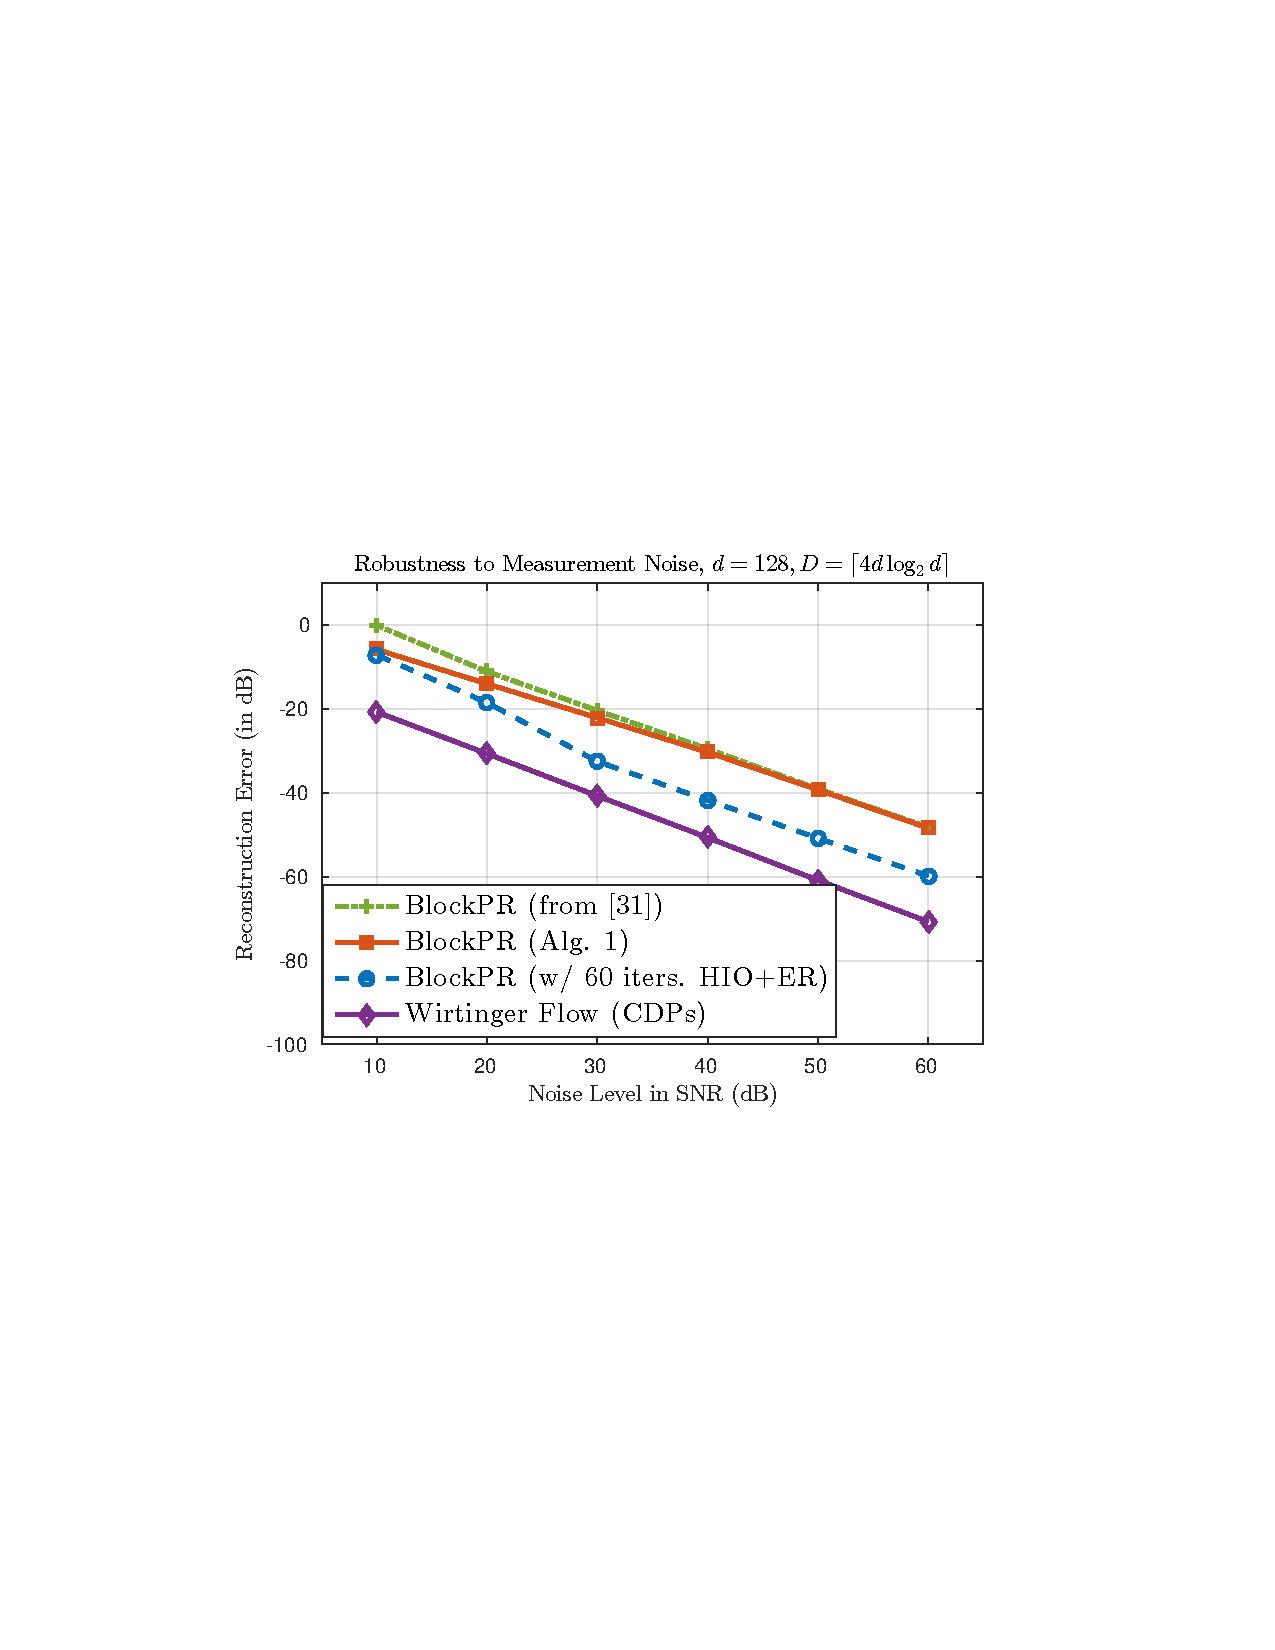
\includegraphics[clip=true, trim = 1.5in 3.5in 1.5in 3.25in,scale=0.610]{pics/fig2a}
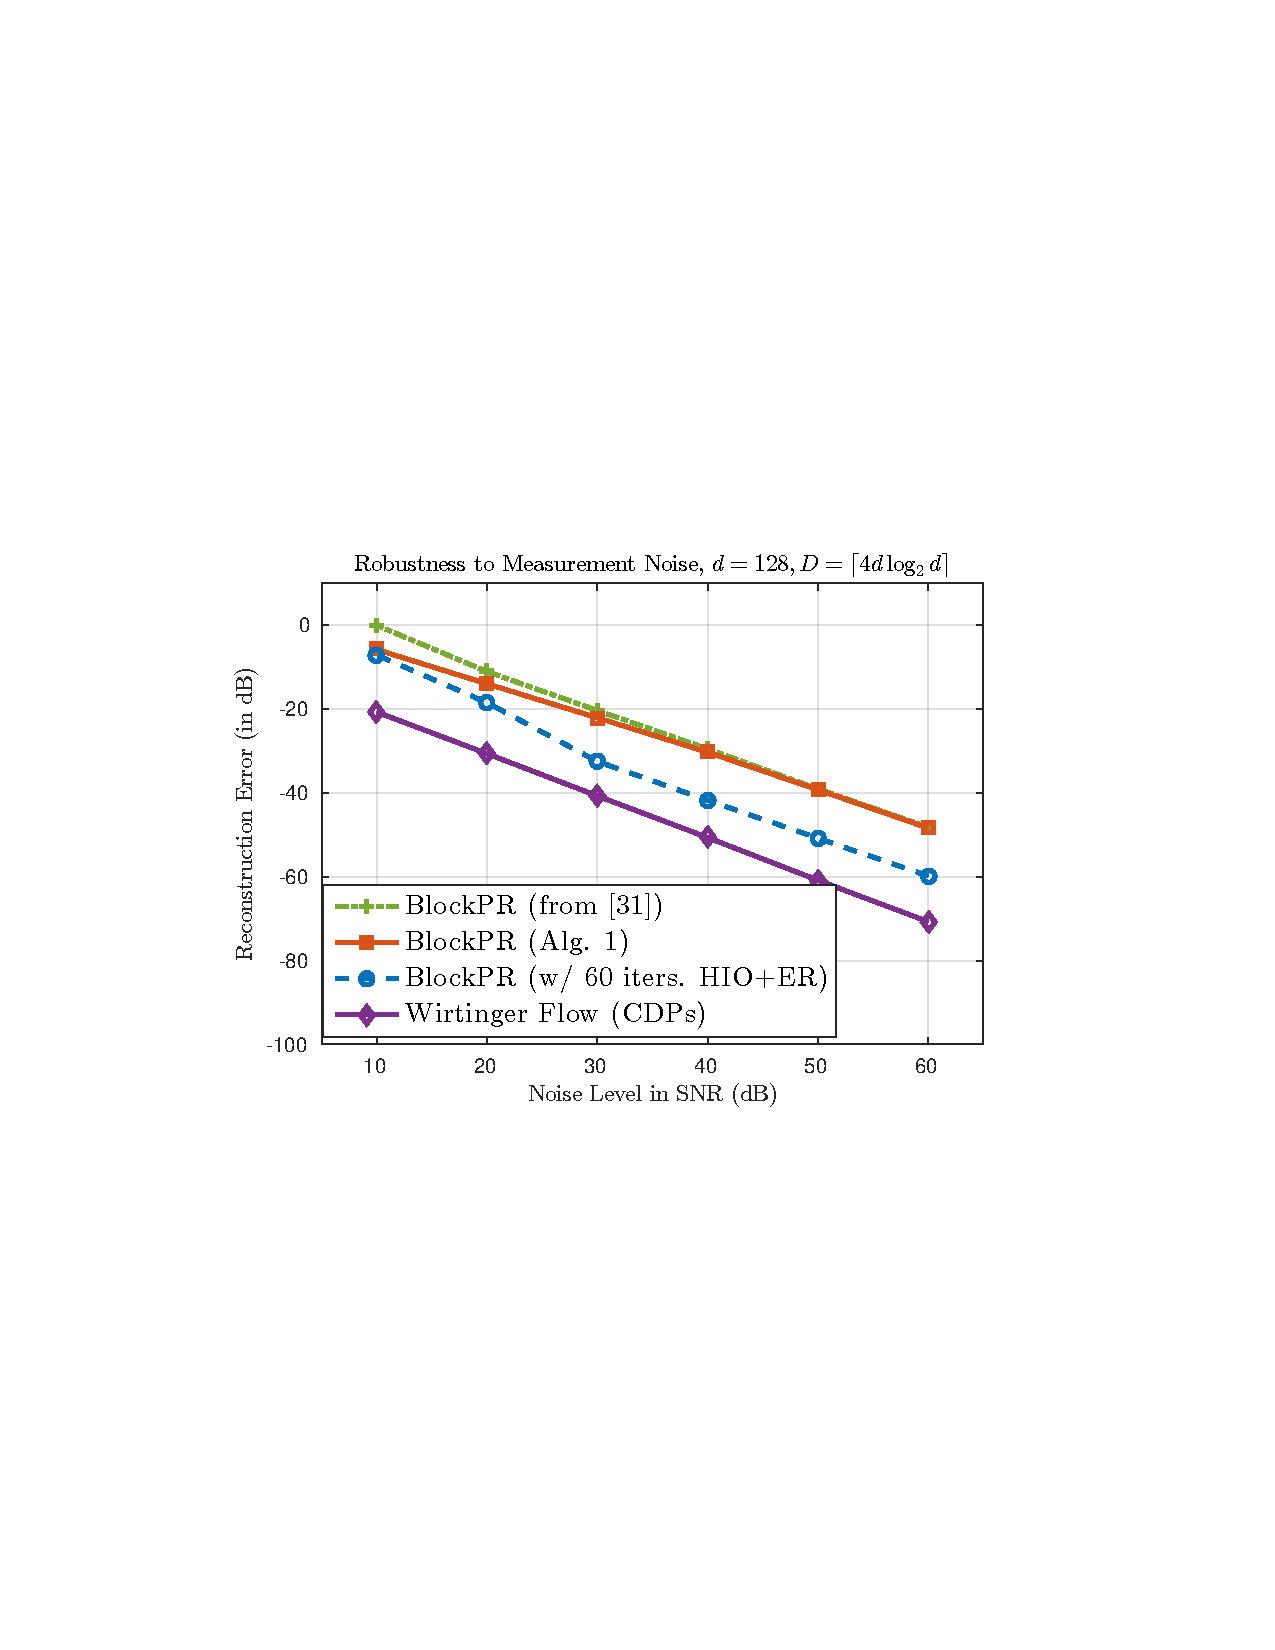
\includegraphics[clip=true, trim = 1.5in 3.5in 1.5in 3.25in, scale=0.80]{pics/fig2a}
\caption{Improved Robustness to Measurement Noise -- Comparing Variants of the {\em BlockPR}
algorithm}
\label{fig:eig_vs_greedy}
\end{subfigure}

\begin{subfigure}[b]{0.8\textwidth}
\centering
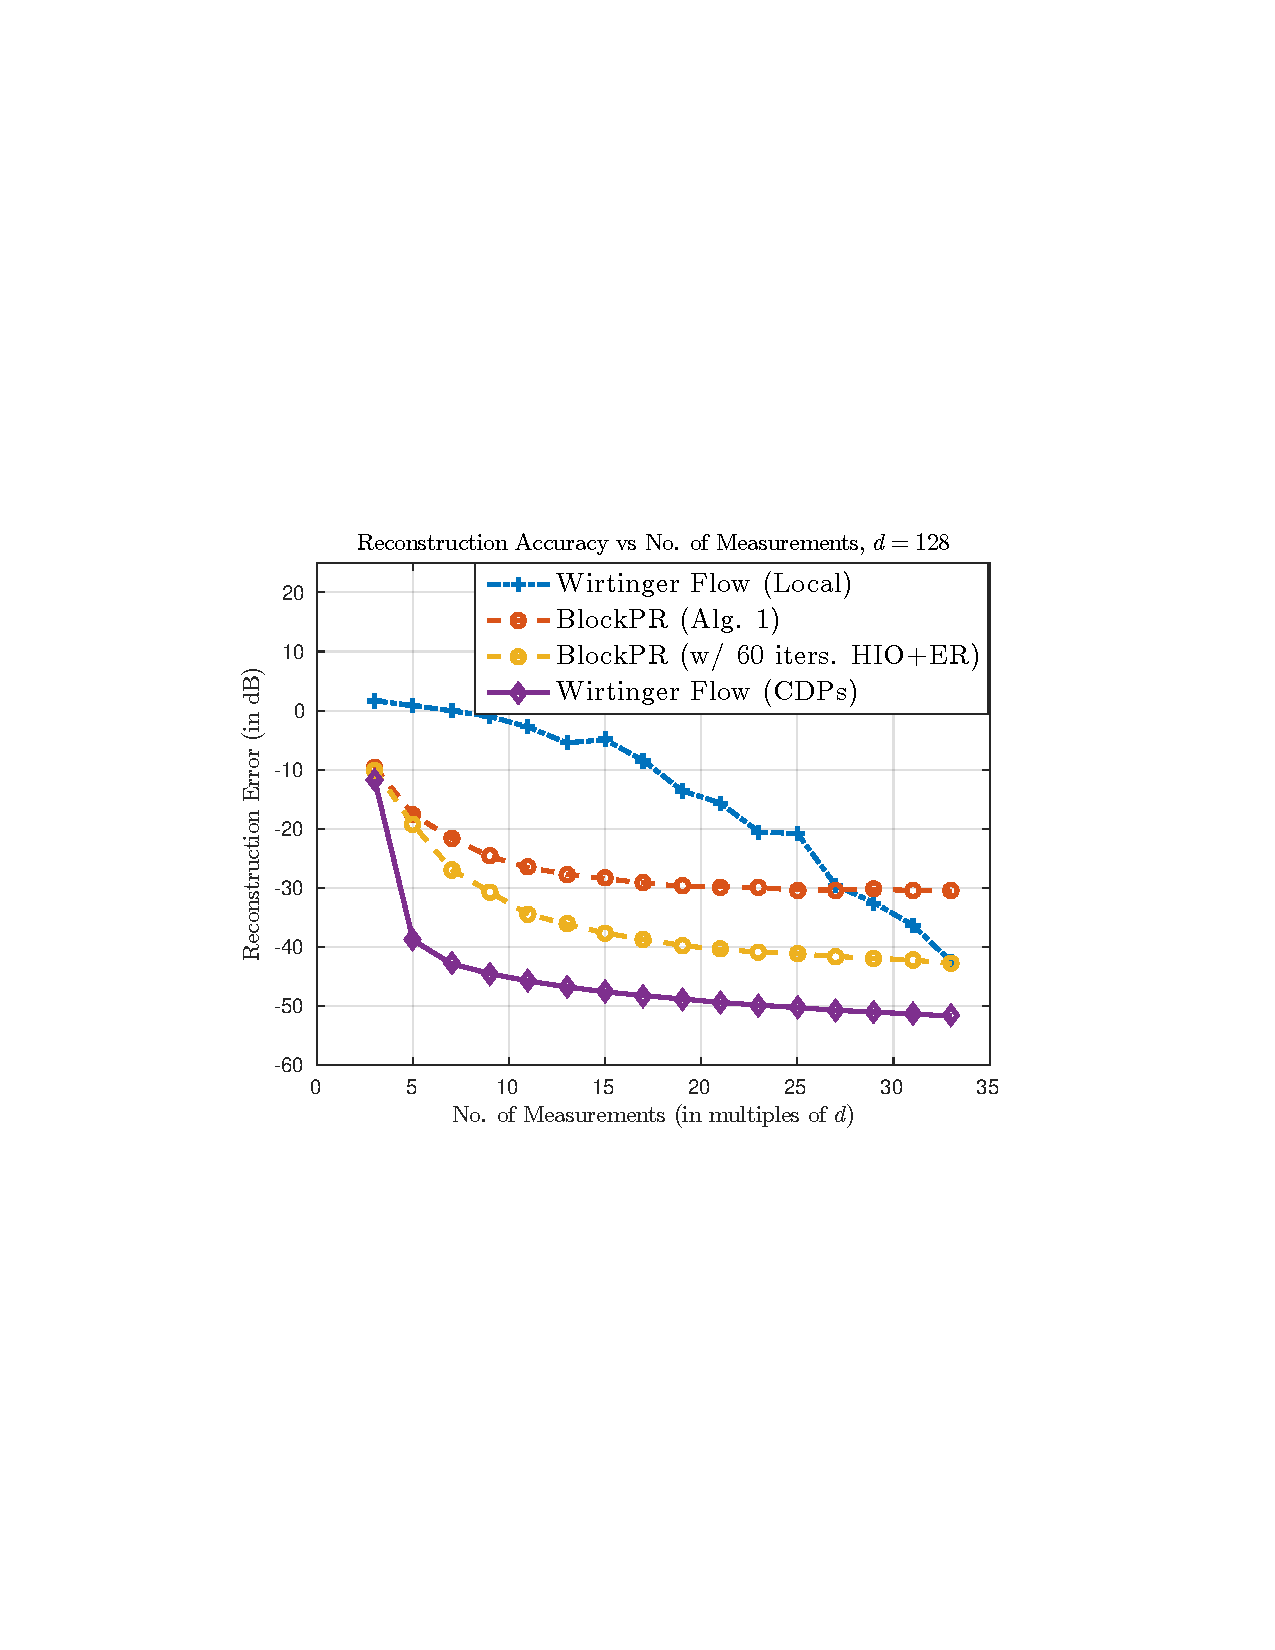
\includegraphics[trim = 1.5in 3.5in 1.5in 3.25in,scale=0.8]{pics/fig2b}
\caption{Reconstruction Error vs. No. of Measurements; (Reconstruction at $40$dB SNR)}
\label{fig:WF_meas}
\end{subfigure}
\caption{Robust Phase Retrieval -- Local vs. Global Measurements}
\label{fig:WF}
\end{figure}
%


%SHOW PLOTS HERE, AND MENTION BRIEFLY THAT WE ARE TAKING THE MEAN OF THE DELTA MAGNITUDE ESTIMATES FOR EACH 
%$|(x_0)_j|$ PRODUCED BY THE TOP EIGENVECTORS OF $D_{j-\delta+1}, \dots, D_j$ IN OUR BETTER IMPLEMENTATION.  IN ADDITION, POST PROCESSING WITH <= 100 ITERATIONS OF ALTERNATING PROJECTIONS IS ALSO USED TO FURTHER IMPROVE OUR FINAL NUMERICAL NOISE ROBUSTNESS...\\
\subsection{Experiments with Measurements from Example 2 of \S \ref{sec:MeasMatrix}}
\label{sec:SparseMeasureMasks}

We begin by presenting results in Fig.~\ref{fig:eig_vs_greedy} demonstrating the improved noise
robustness of the proposed method over the formulation in \cite{IVW2015_FastPhase}. Recall that
\cite{IVW2015_FastPhase} uses a greedy angular synchronization method instead of the
eigenvector-based procedure analyzed in this paper. Fig.~\ref{fig:eig_vs_greedy} plots the
reconstruction error when recovering a $d=128$ length complex Gaussian test signal using $D=\lceil
4d\log_2 d\rceil$ measurements at different added noise levels. As mentioned above,
the local correlation measurements described in Example 2 of Section \ref{sec:MeasMatrix} are
utilized in this plot and in all the ensuing experiments in this subsection unless otherwise
indicated. Three variants of the proposed algorithm are plotted in Fig.~\ref{fig:eig_vs_greedy}:
\begin{enumerate}
    \item an implementation of Algorithm \ref{alg:phaseRetrieval1} (denoted by $\square$'s),
%    \item an implementation of Algorithm \ref{alg:phaseRetrieval1} with the improved magnitude estimation
%        procedure detailed in \S \ref{sec:MagEstImpNumerical} (with $s=1$ and using the average of the obtained $\tilde D_{j\prime}$
%        block magnitude estimates) and post-processed using $100$ iterations of the {\em
%        Gerchberg--Saxton} (or Error Reduction -- ER)
%        alternating projection algorithm (denoted by $\circ$'s), and 
    \item an implementation of Algorithm \ref{alg:phaseRetrieval1} post-processed using 
        $60$ iterations of the Hybrid Input--Output (HIO) and Error Reduction (ER) algorithms
        (implemented in two successive sets, with each set consisting of $20$ iterations of HIO followed 
        by $10$ ER iterations; denoted by $\circ$'s), and 
    \item the algorithmic implementation from \cite{IVW2015_FastPhase} (denoted by $+$'s). 
\end{enumerate}
%
We see that the eigenvector-based angular synchronization method proposed in this paper provides
more accurate reconstructions -- especially at low SNRs -- over the greedy angular synchronization
of \cite{IVW2015_FastPhase}. Moreover, post-processing using the HIO+ER algorithms as detailed above yields
a significant improvement in reconstruction errors over the two other variants. For reference, we also
include reconstruction errors with the {\em Wirtinger Flow} algorithm (denoted by $\Diamond$'s) when
using ({\em global}) coded diffraction pattern (CDP) measurements. Specifically, we use $2\delta-1$
(with $\delta = 2\log_2d = 14$) octanary modulations/codes as described in \cite[\S 1.5,
(1.9)]{Candes2014WF} to construct the CDP measurements. Clearly, using global measurements such as
coded diffraction patterns provides superior noise tolerance; however, they are not applicable to
the local measurement model considered here.  Indeed, when the {\em Wirtinger Flow} algorithm is
used with local measurements such as those described in this paper, the noise tolerance
significantly deteriorates. Fig. \ref{fig:WF_meas} illustrates this phenomenon by plotting the
reconstruction error in recovering a $d=128$ length complex Gaussian test signal at $40$~dB SNR when
using different numbers of measurements, $D$. {\em Wirtinger flow}, for example, requires a large
number of local measurements before returning accurate reconstructions. 
%We conjecture that the spectral initialization used in {\em
%Wirtinger Flow} and devised for
%global measurements (random Gaussian and coded diffraction pattern measurements) is less effective
%when applied to local measurements such as those considered in this paper. 
The wide disparity in reconstruction accuracy between local and global measurements for {\em
Wirtinger Flow} illustrates the significant challenge in phase retrieval from local measurements.
Furthermore, we see that the {\em BlockPR} method proposed in this paper is more noise tolerant than
{\em Wirtinger Flow} for local measurements.
%
\begin{figure}[hbtp]
\centering
\begin{subfigure}[b]{0.510\textwidth}
\centering
%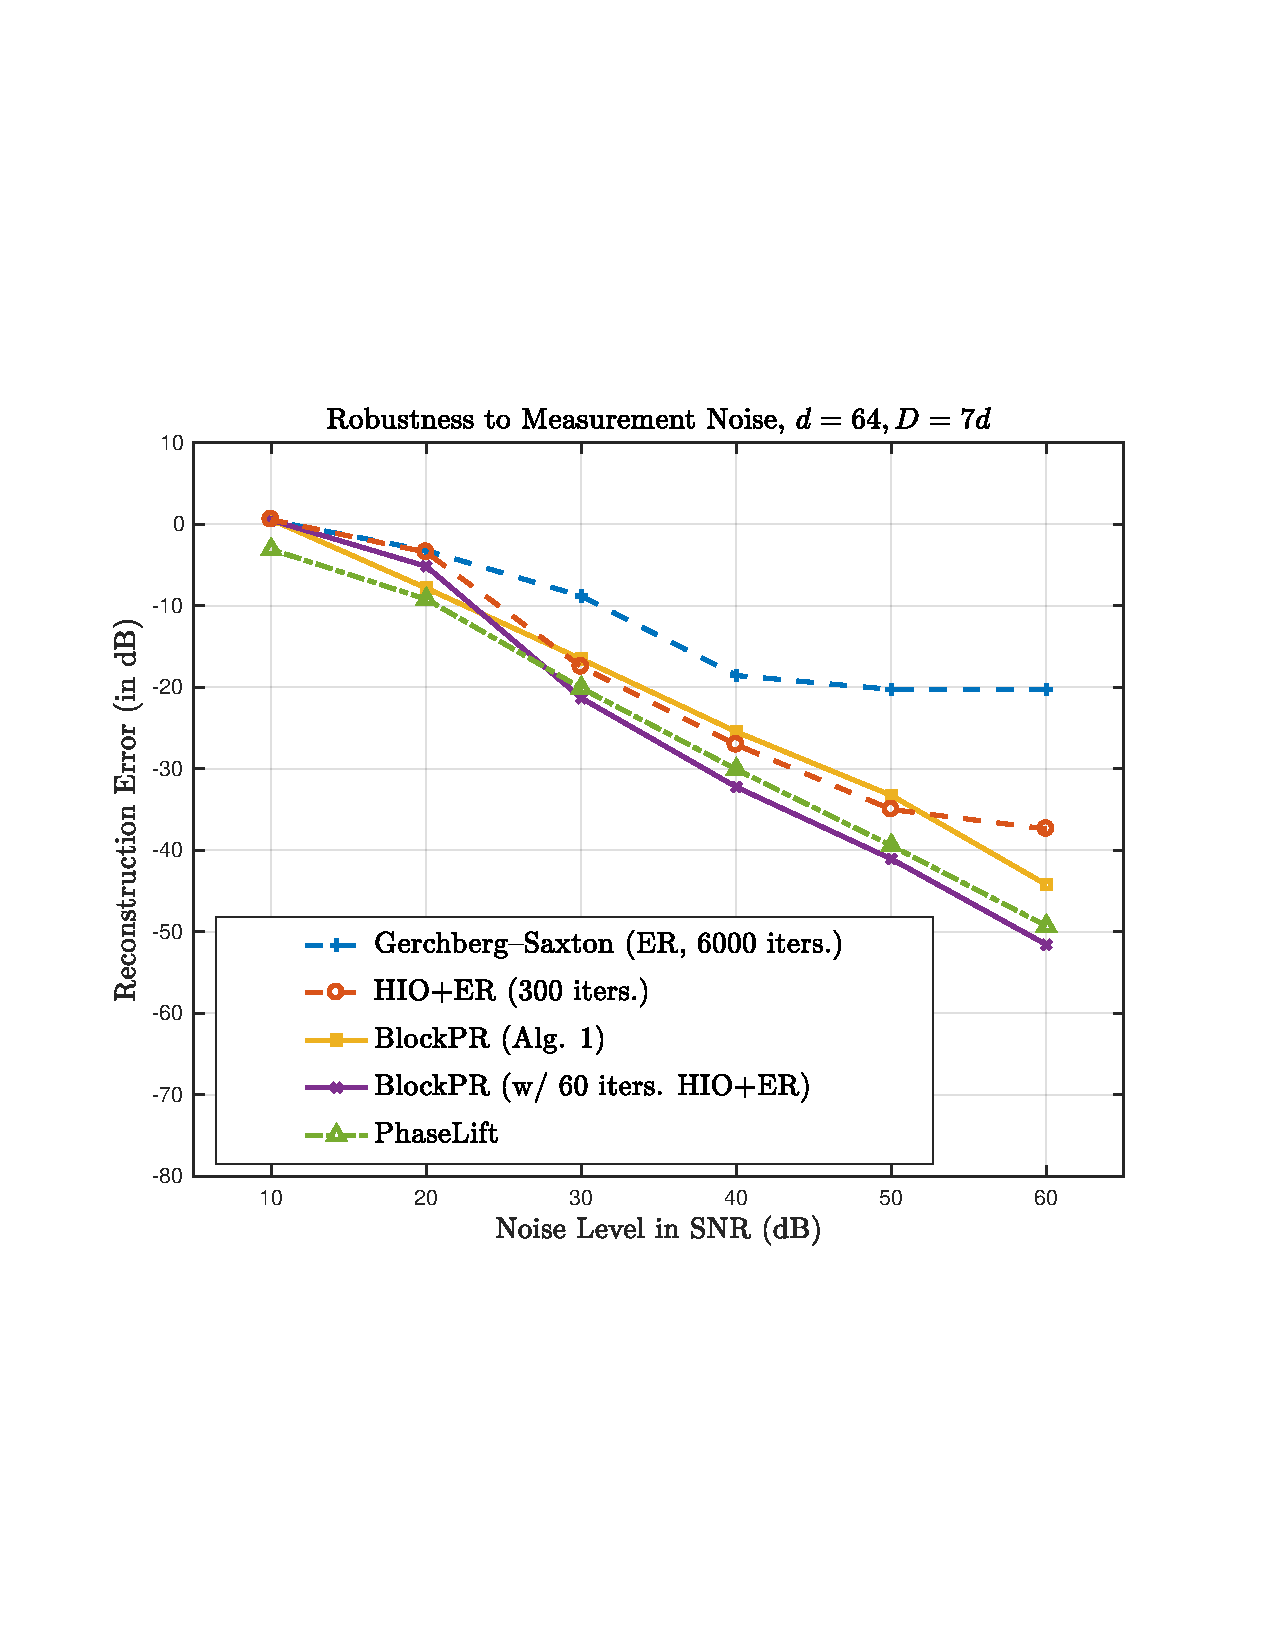
\includegraphics[clip=true, trim = 0.75in 2.75in 1in 2.5in,scale=0.45]{pics/fig3a}
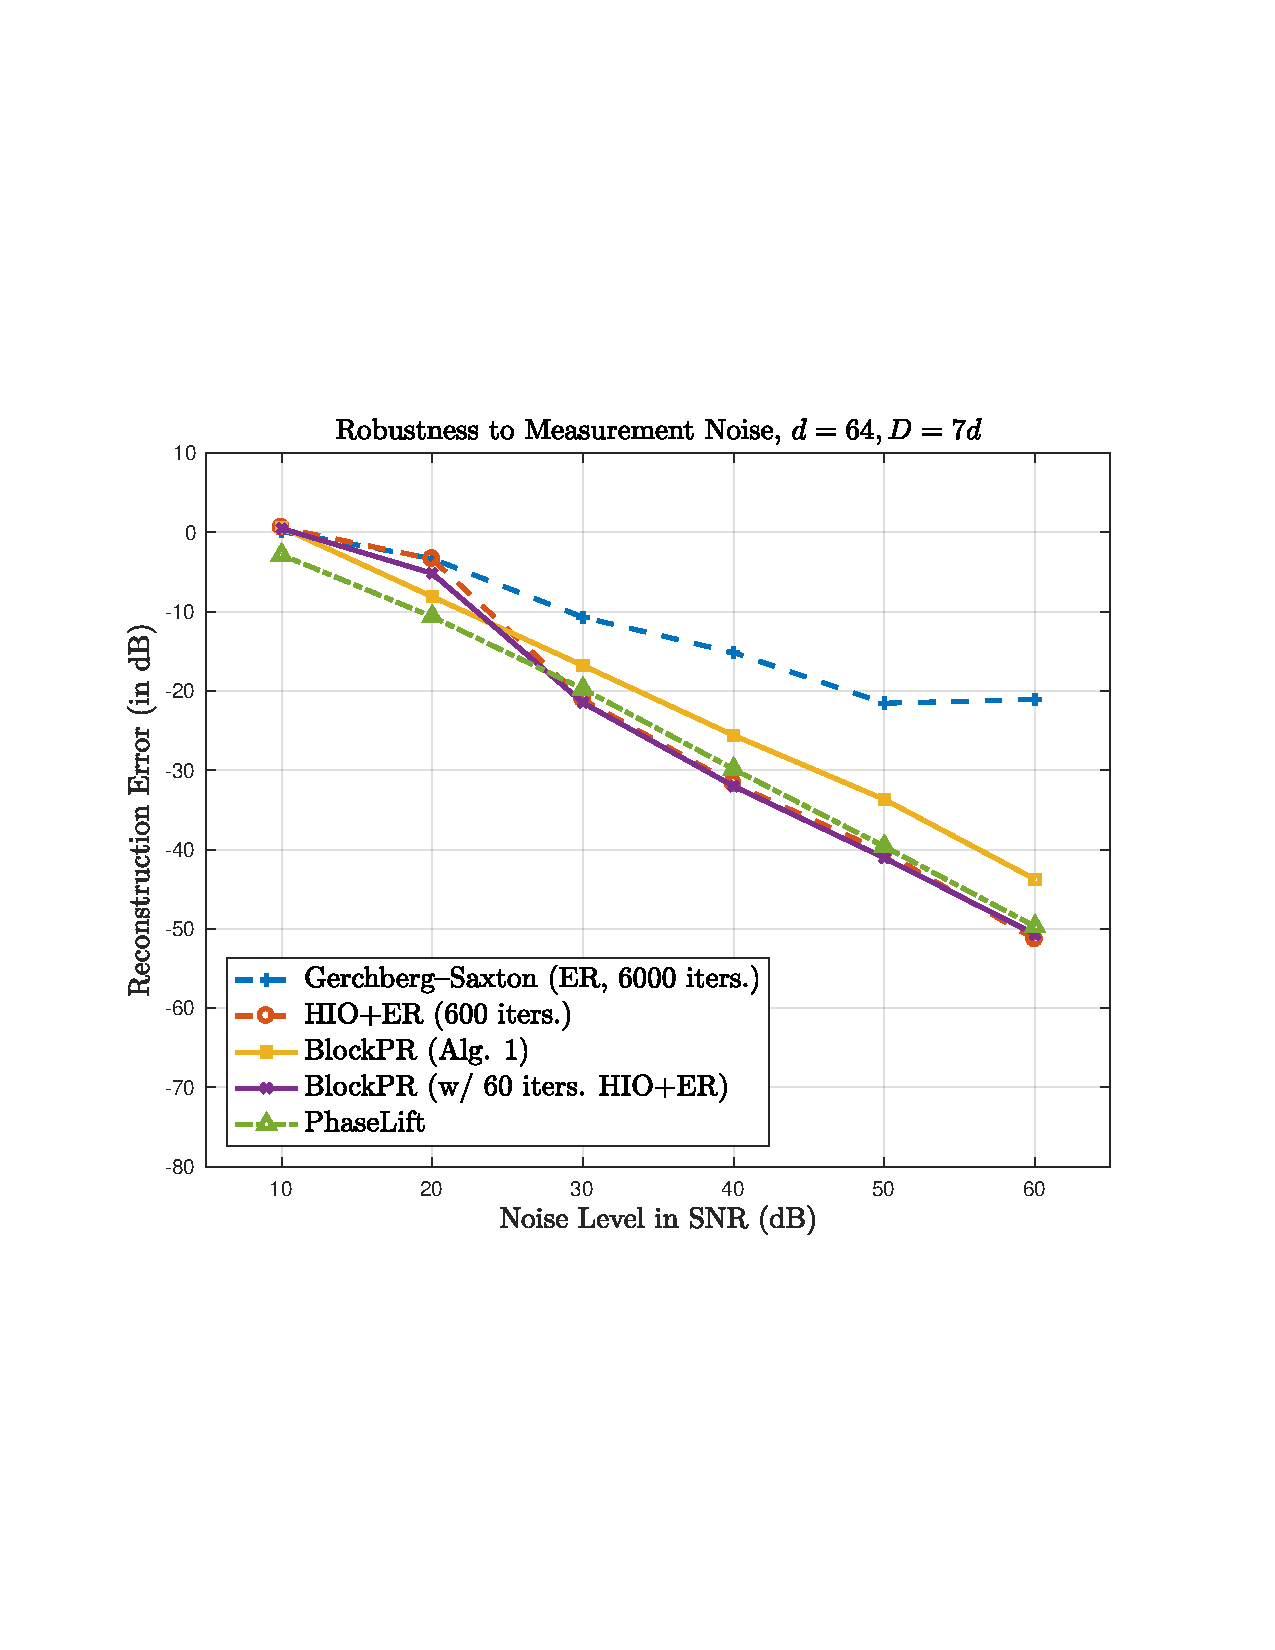
\includegraphics[clip=true, trim = 0.75in 2.75in 1in 2.5in,scale=0.45]{pics/robustness_600a}
\caption{Using $D=7d$ measurements.}
\label{fig:noise-7d}
\end{subfigure}
\hfill
\begin{subfigure}[b]{0.480\textwidth}
\centering
%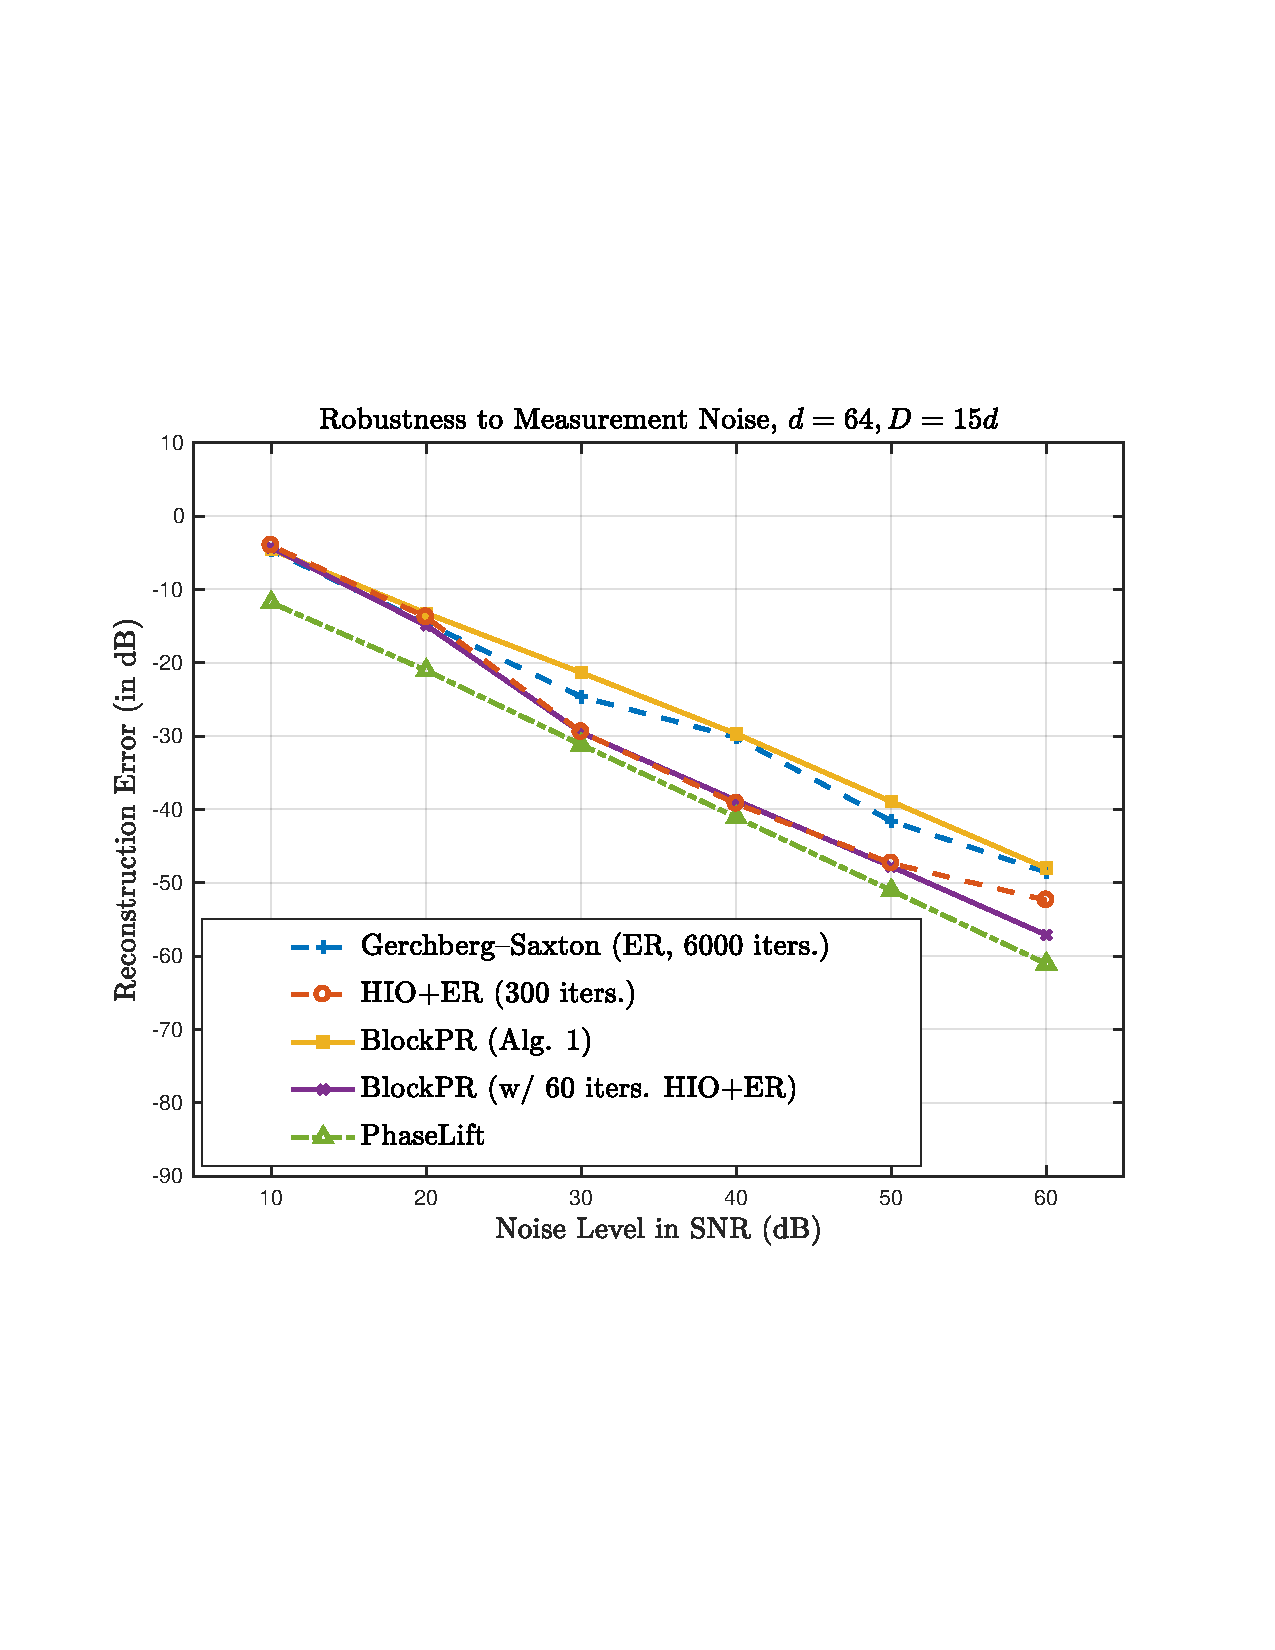
\includegraphics[clip=true, trim = 0.75in 2.75in 1in 2.5in,scale=0.45]{pics/fig3b}
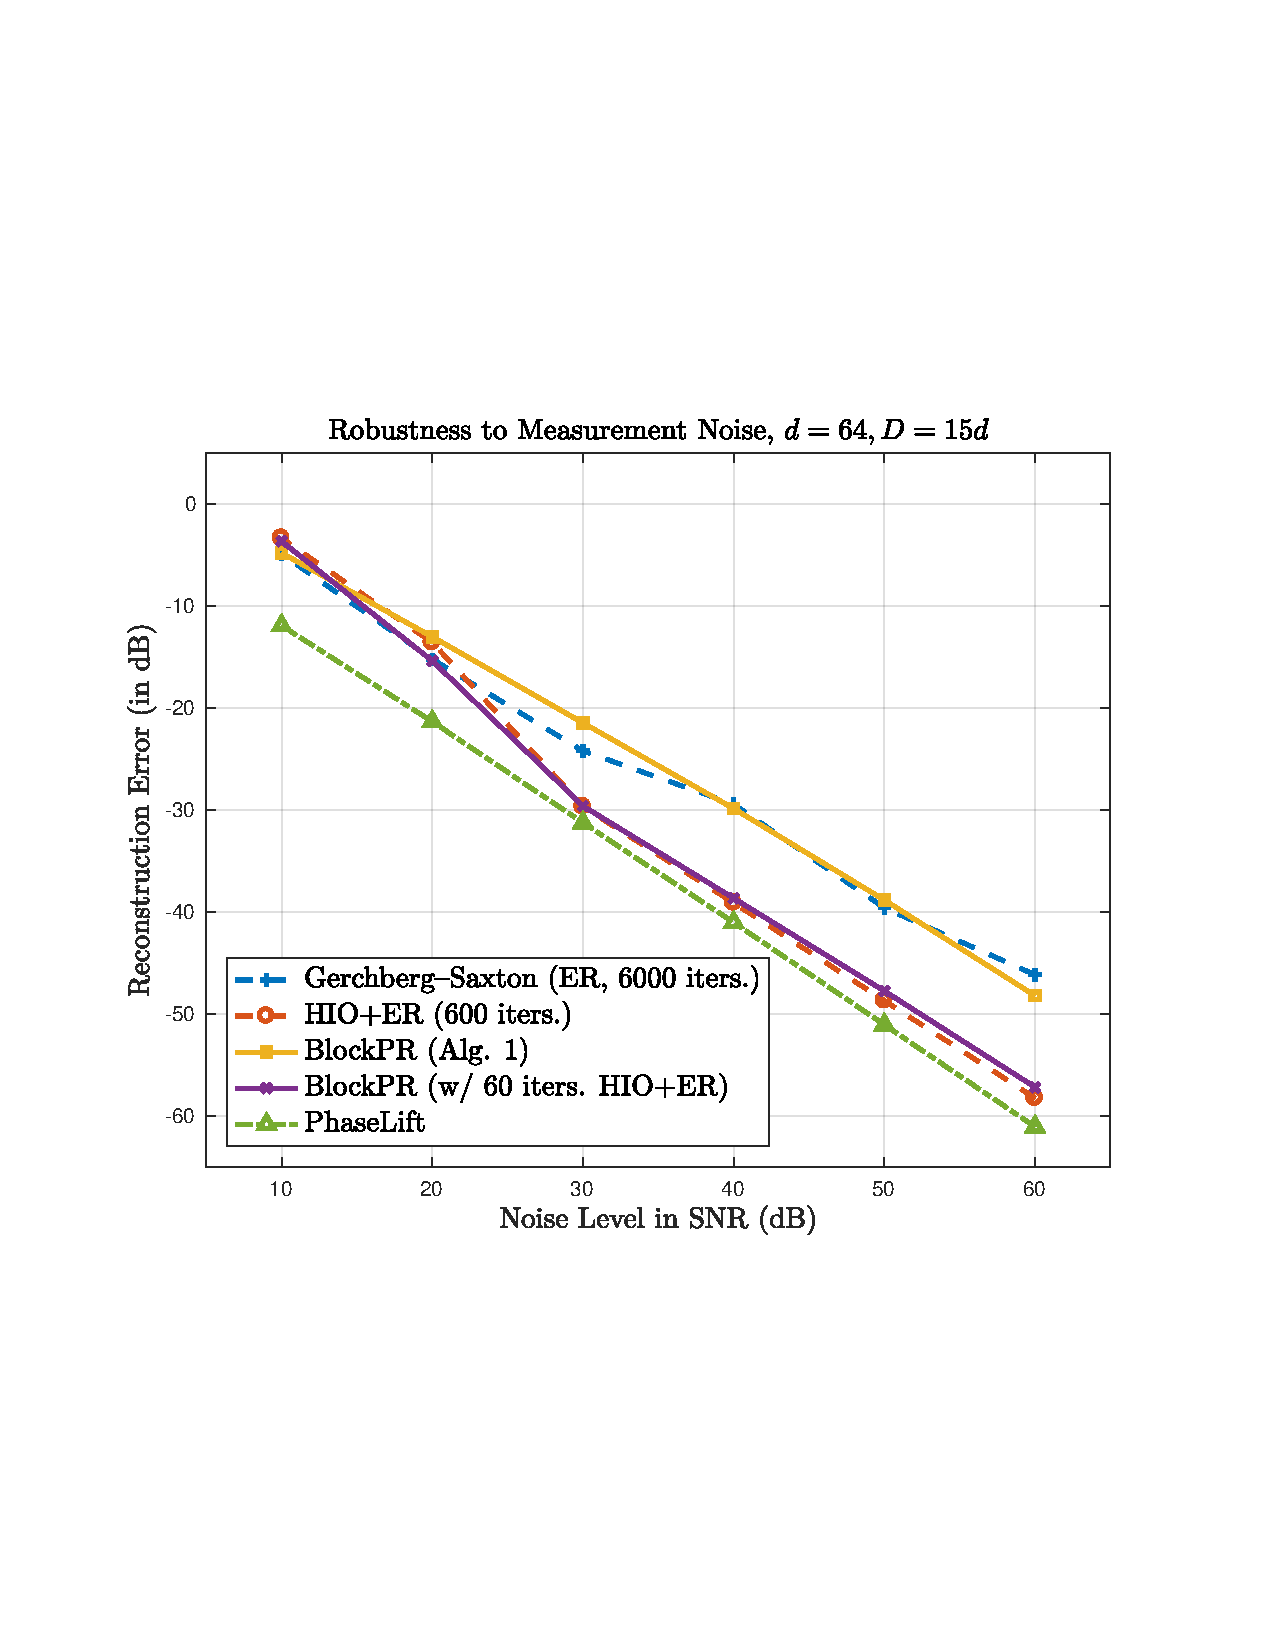
\includegraphics[clip=true, trim = 0.75in 2.75in 1in 2.5in,scale=0.45]{pics/robustness_600b}
\caption{Using $D=15d$ measurements.}
\label{fig:noise-15d}
\end{subfigure}\vspace{0.1in} \\
\begin{subfigure}[b]{0.510\textwidth}
\centering
%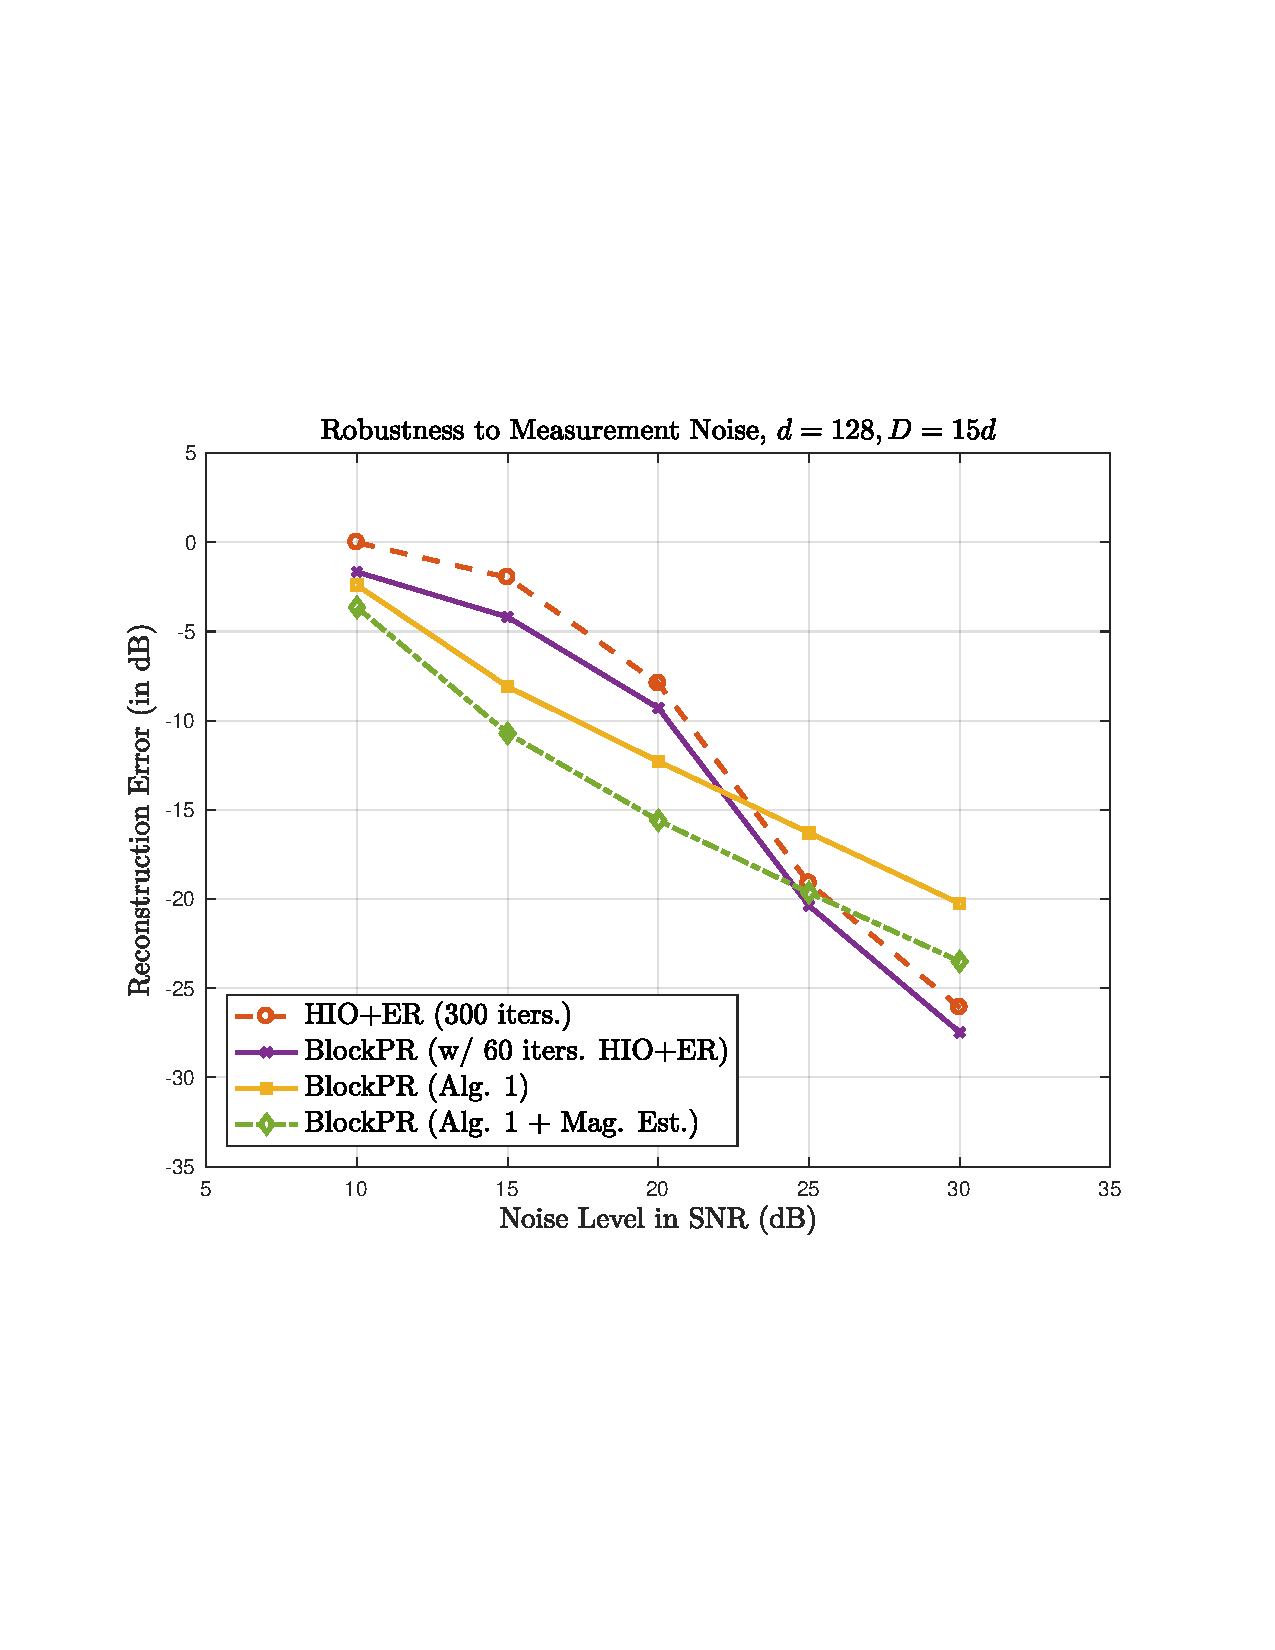
\includegraphics[clip=true, trim = 0.75in 2.75in 1in 2.5in,scale=0.45]{pics/fig3c}
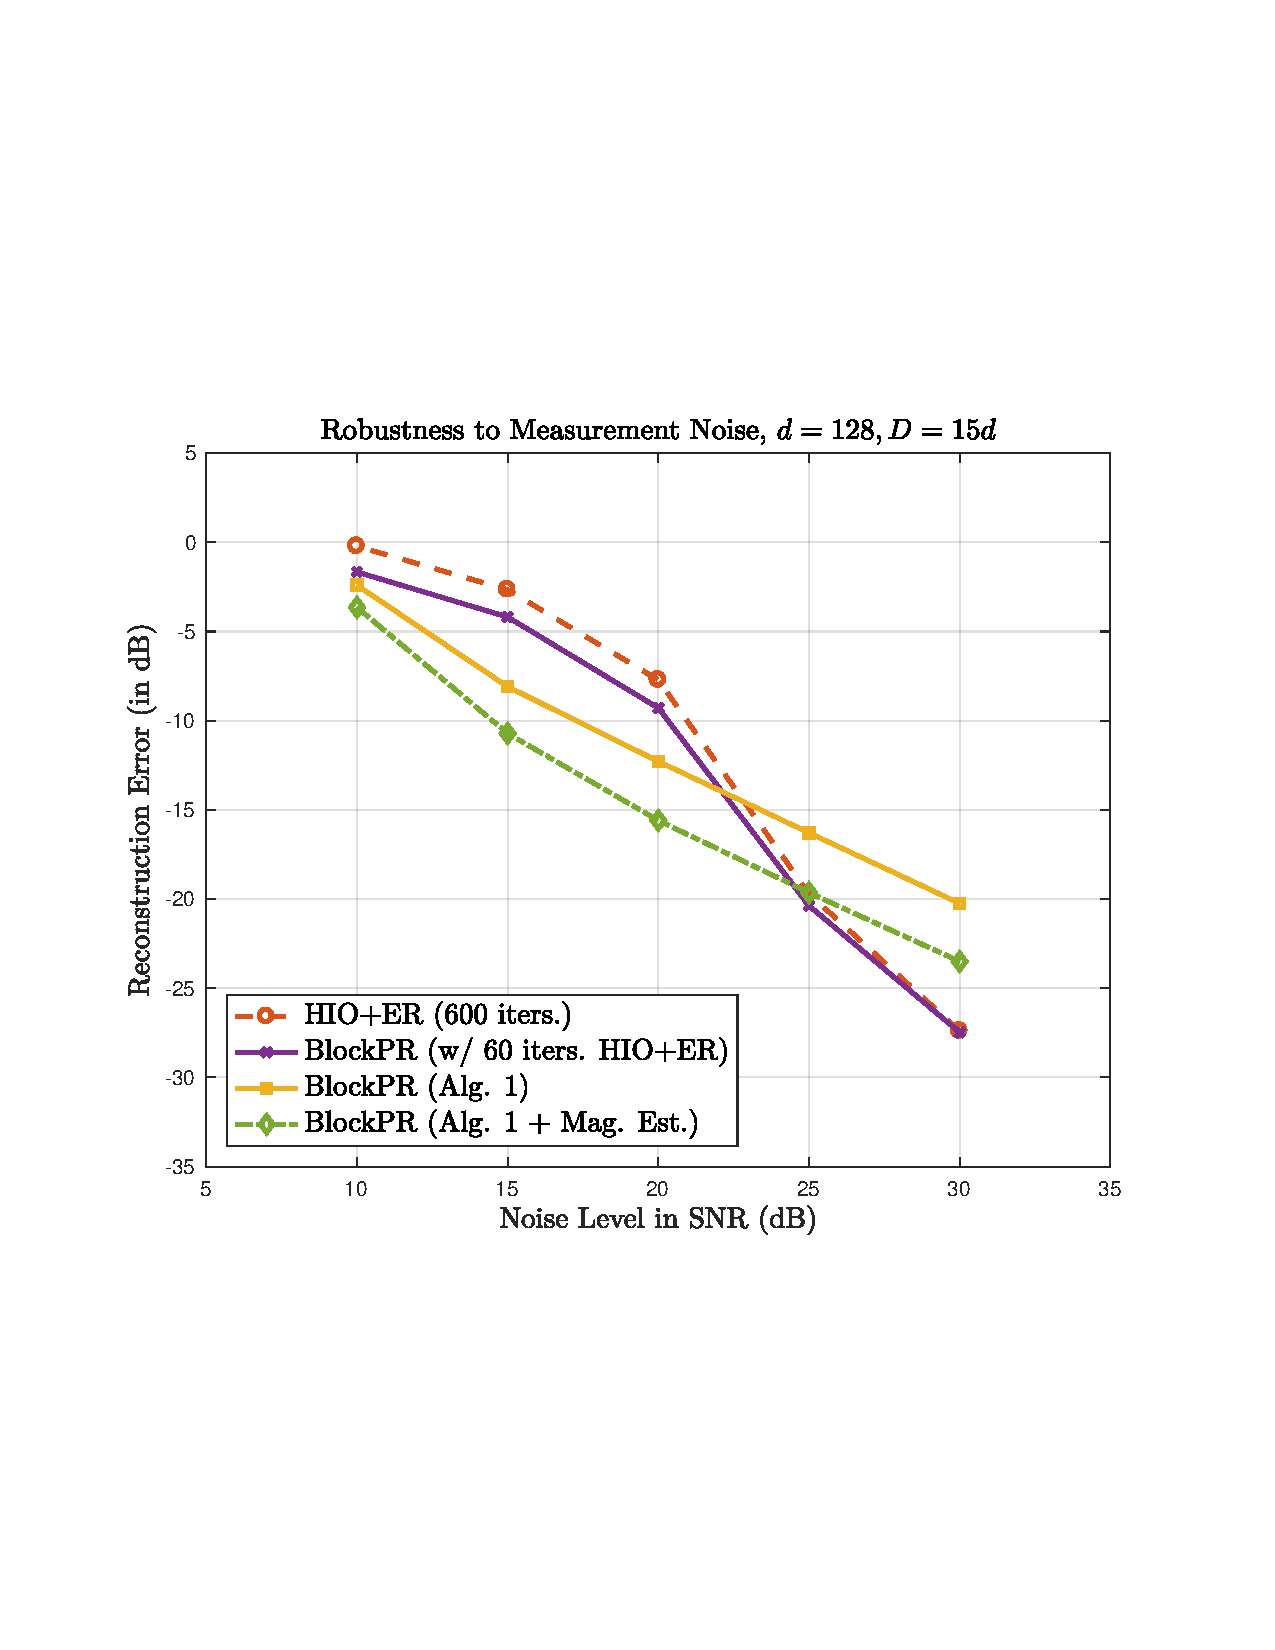
\includegraphics[clip=true, trim = 0.75in 2.75in 1in 2.5in,scale=0.45]{pics/robustness_600c}
\caption{Low SNR Simulations: Using $D=15d$ measurements, Problem Size $d=128$}
\label{fig:lowsnr_128}
\end{subfigure}
\hfill
\begin{subfigure}[b]{0.480\textwidth}
\centering
%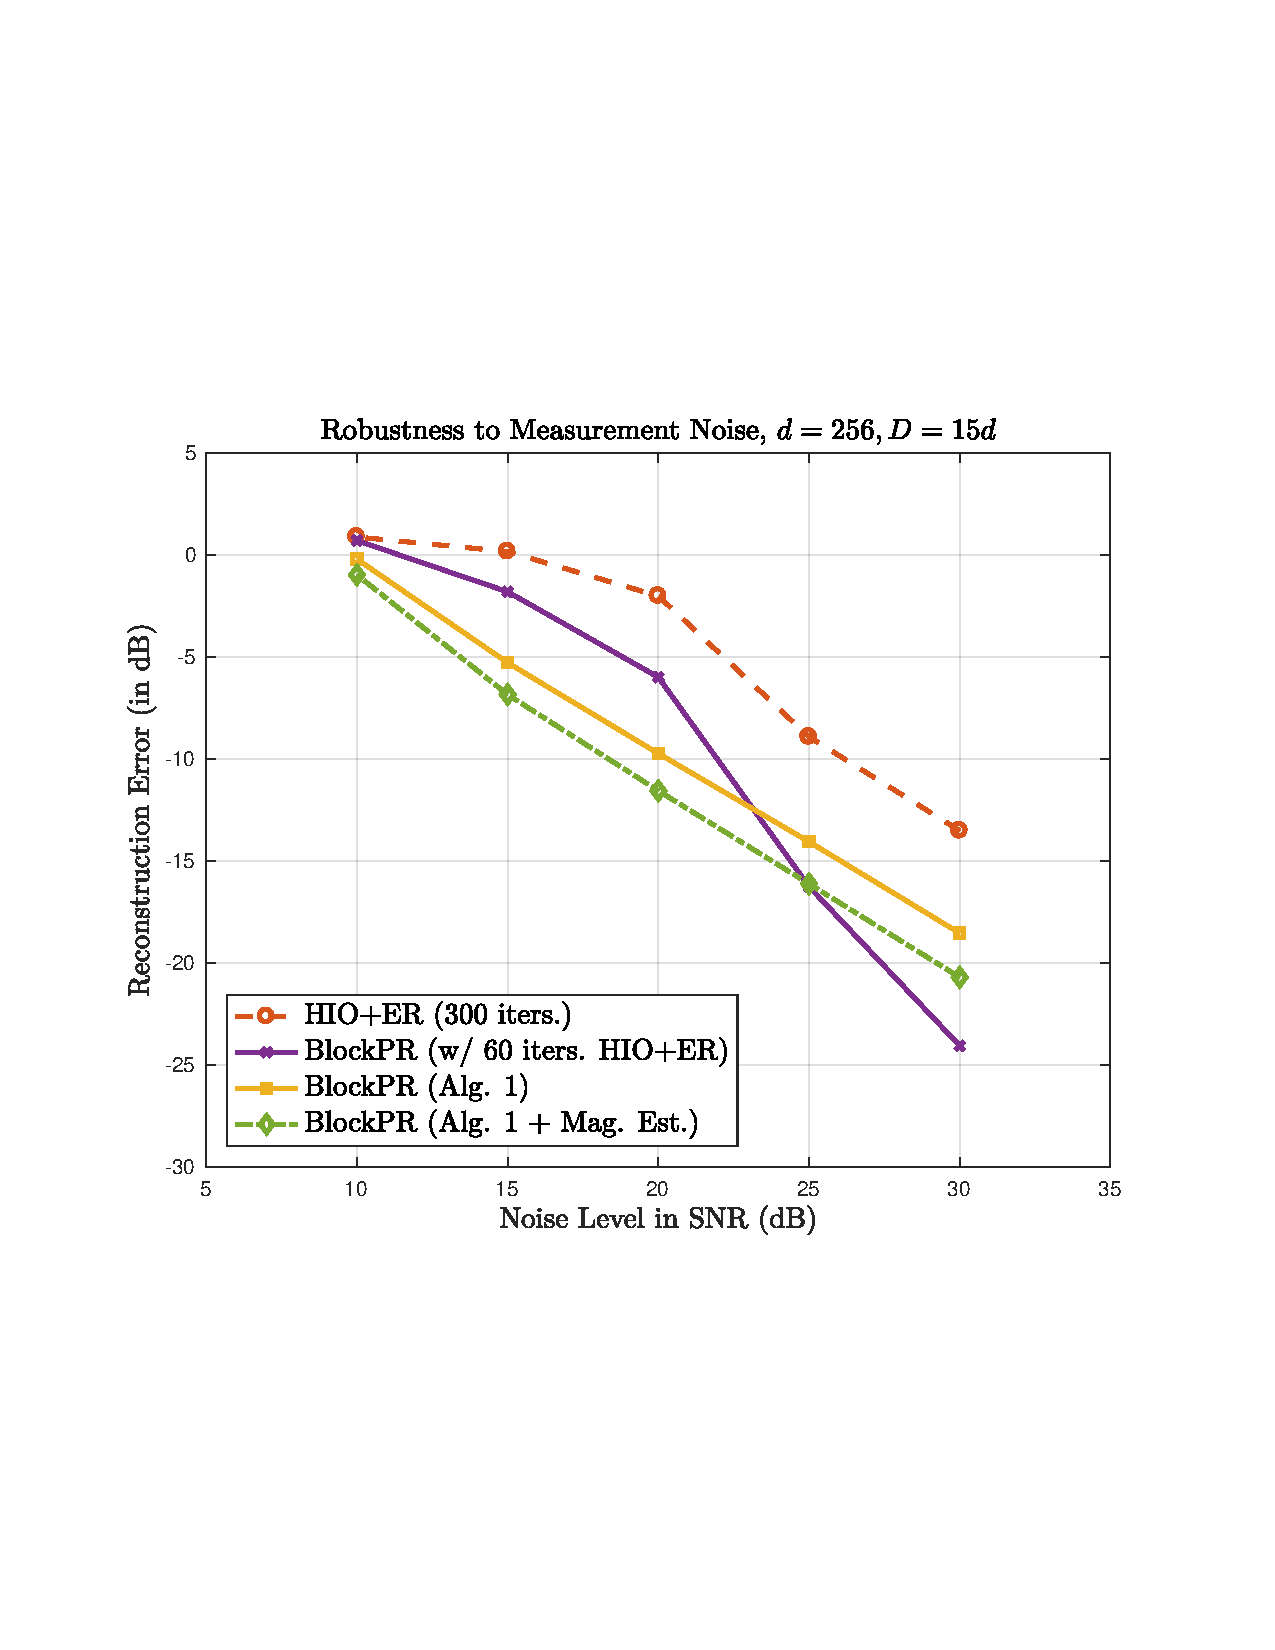
\includegraphics[clip=true, trim = 0.75in 2.75in 1in 2.5in,scale=0.45]{pics/fig3d}
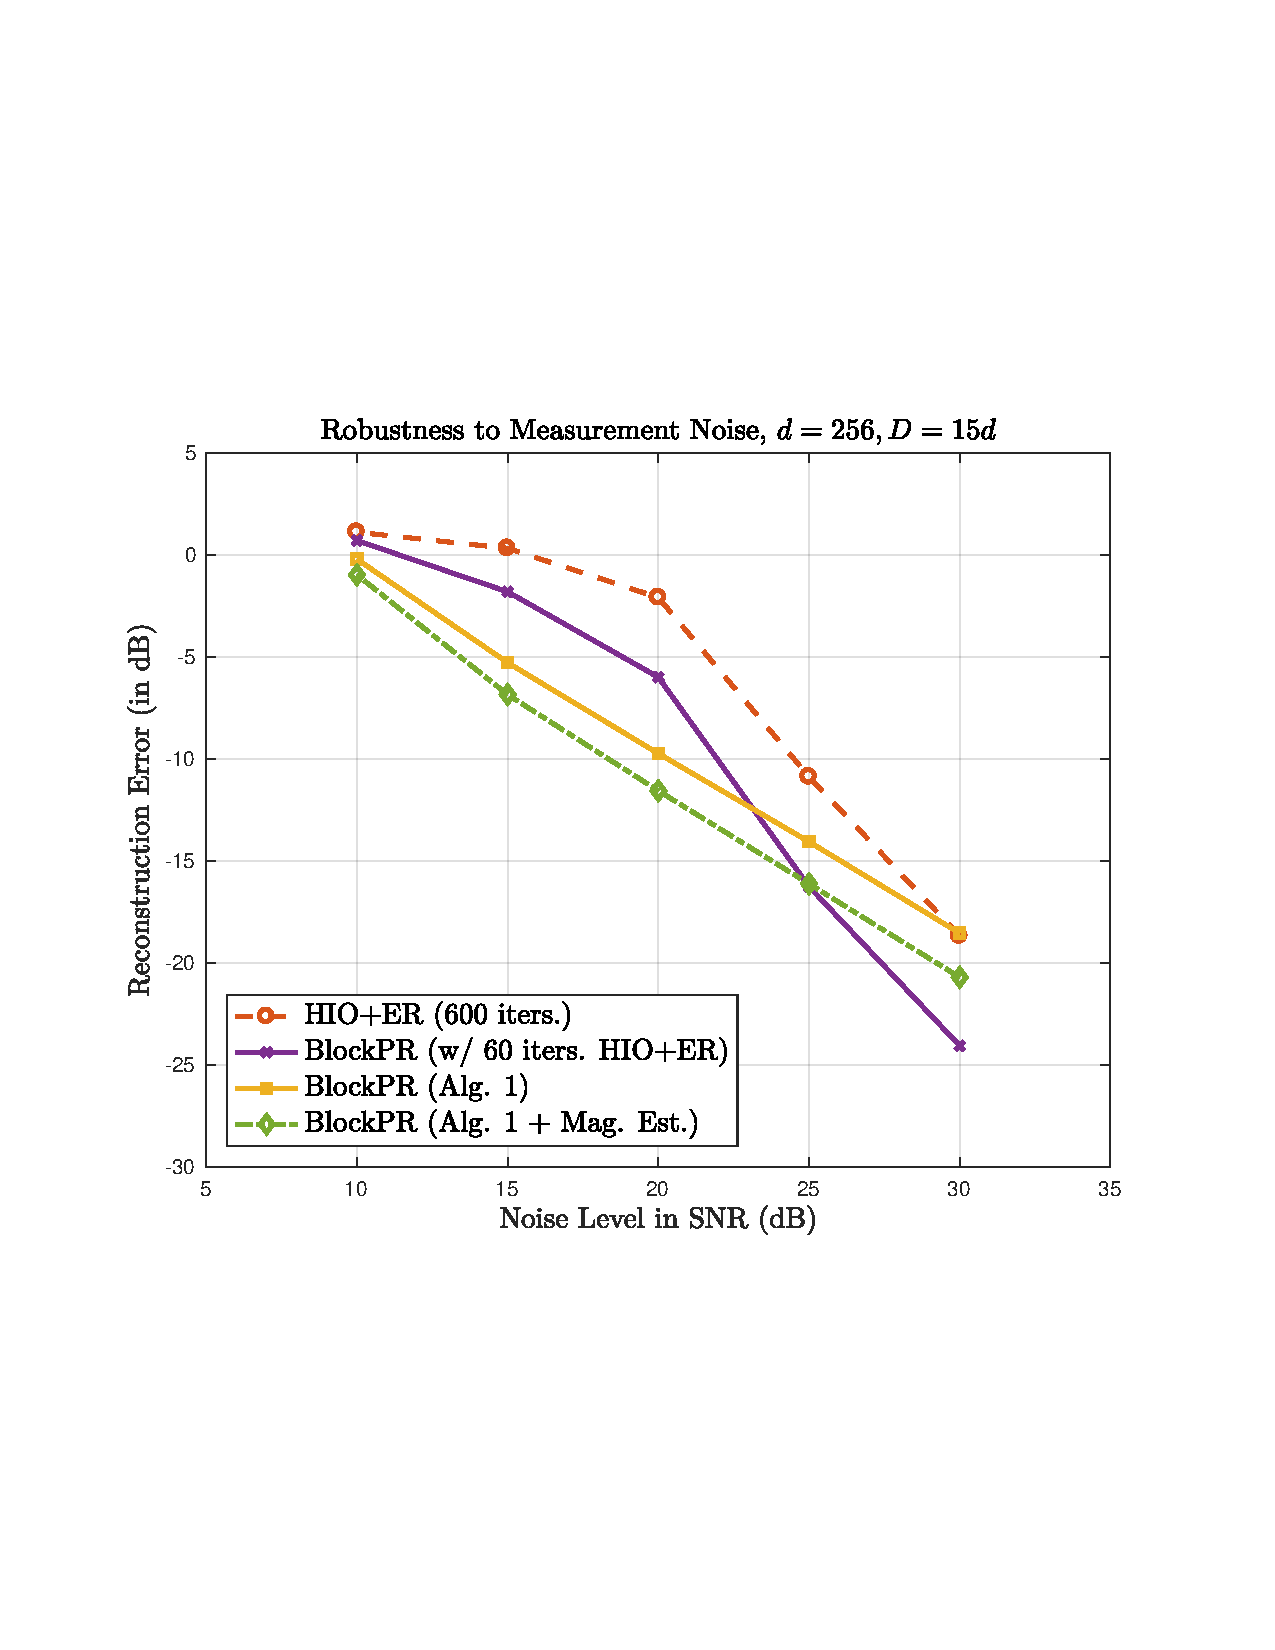
\includegraphics[clip=true, trim = 0.75in 2.75in 1in 2.5in,scale=0.45]{pics/robustness_600d}
\caption{Low SNR Simulations: Using $D=15d$ measurements, Problem Size $d=256$}
\label{fig:lowsnr_256}
\end{subfigure}
\caption{Robustness to measurement noise -- Phase Retrieval from 
deterministic local correlation measurements.}
\label{fig:noise-local}
\end{figure}
%
%\subsection{Robustness to Measurement Noise}
%\label{sec:numeval-noise}

Given the weaker performance of {\em Wirtinger Flow} with local measurements, we now restrict our attention to the empirical evaluation of the proposed method (Alg. \ref{alg:phaseRetrieval1}, as well as the post-processed variant (with HIO+ER iterations)) against {\em PhaseLift} and alternating projection algorithms. Although numerical simulations suggest that these methods work with local measurements, we note that (to the best of our knowledge) there are no theoretical recovery or robustness guarantees for these methods and measurements.  The {\em PhaseLift} algorithm was implemented as a trace regularized least-squares problem using CVX \cite{cvx,gb08} -- a package for specifying and solving convex programs in Matlab. We consider two variants from the family of alternating projection methods -- {\em Gerchberg--Saxton} (sometimes referred to as the Error Reduction (ER) algorithm) and Hybrid Input-Output (HIO). For both algorithms, the following two projections were utilized: (i) projection onto the measured magnitudes, and (ii) projection onto the span of the measurement vectors $\{\a_j\}_{j=1}^D$. This formulation as well as other details and connections to convex optimization theory can be found in \cite{bauschke2002phase}. For the ER and HIO implementations, the initial guess was set to be the all-zero vector.\footnote{\ We note that using a random starting guess does not change the qualitative nature of the empirical results.} For the HIO implementation, as is popular practice (see, for example, \cite{fienup1982comparison}) every few ($20$) HIO iterations were followed by a small number of ($10$) ER iterations, with the maximum number of HIO+ER iterations limited to $600$ -- this choice of iteration count ensures convergence of the algorithm (see Fig. \ref{fig:iter_HIOER}) while comparing favorably with the computational cost (see Fig. \ref{fig:exectime}) of the proposed {\em BlockPR} method. For the ER implementation, $6,000$ iterations were necessary to ensure convergence.

%-------------------------------------------------------
\begin{figure}[H]
  \centering
  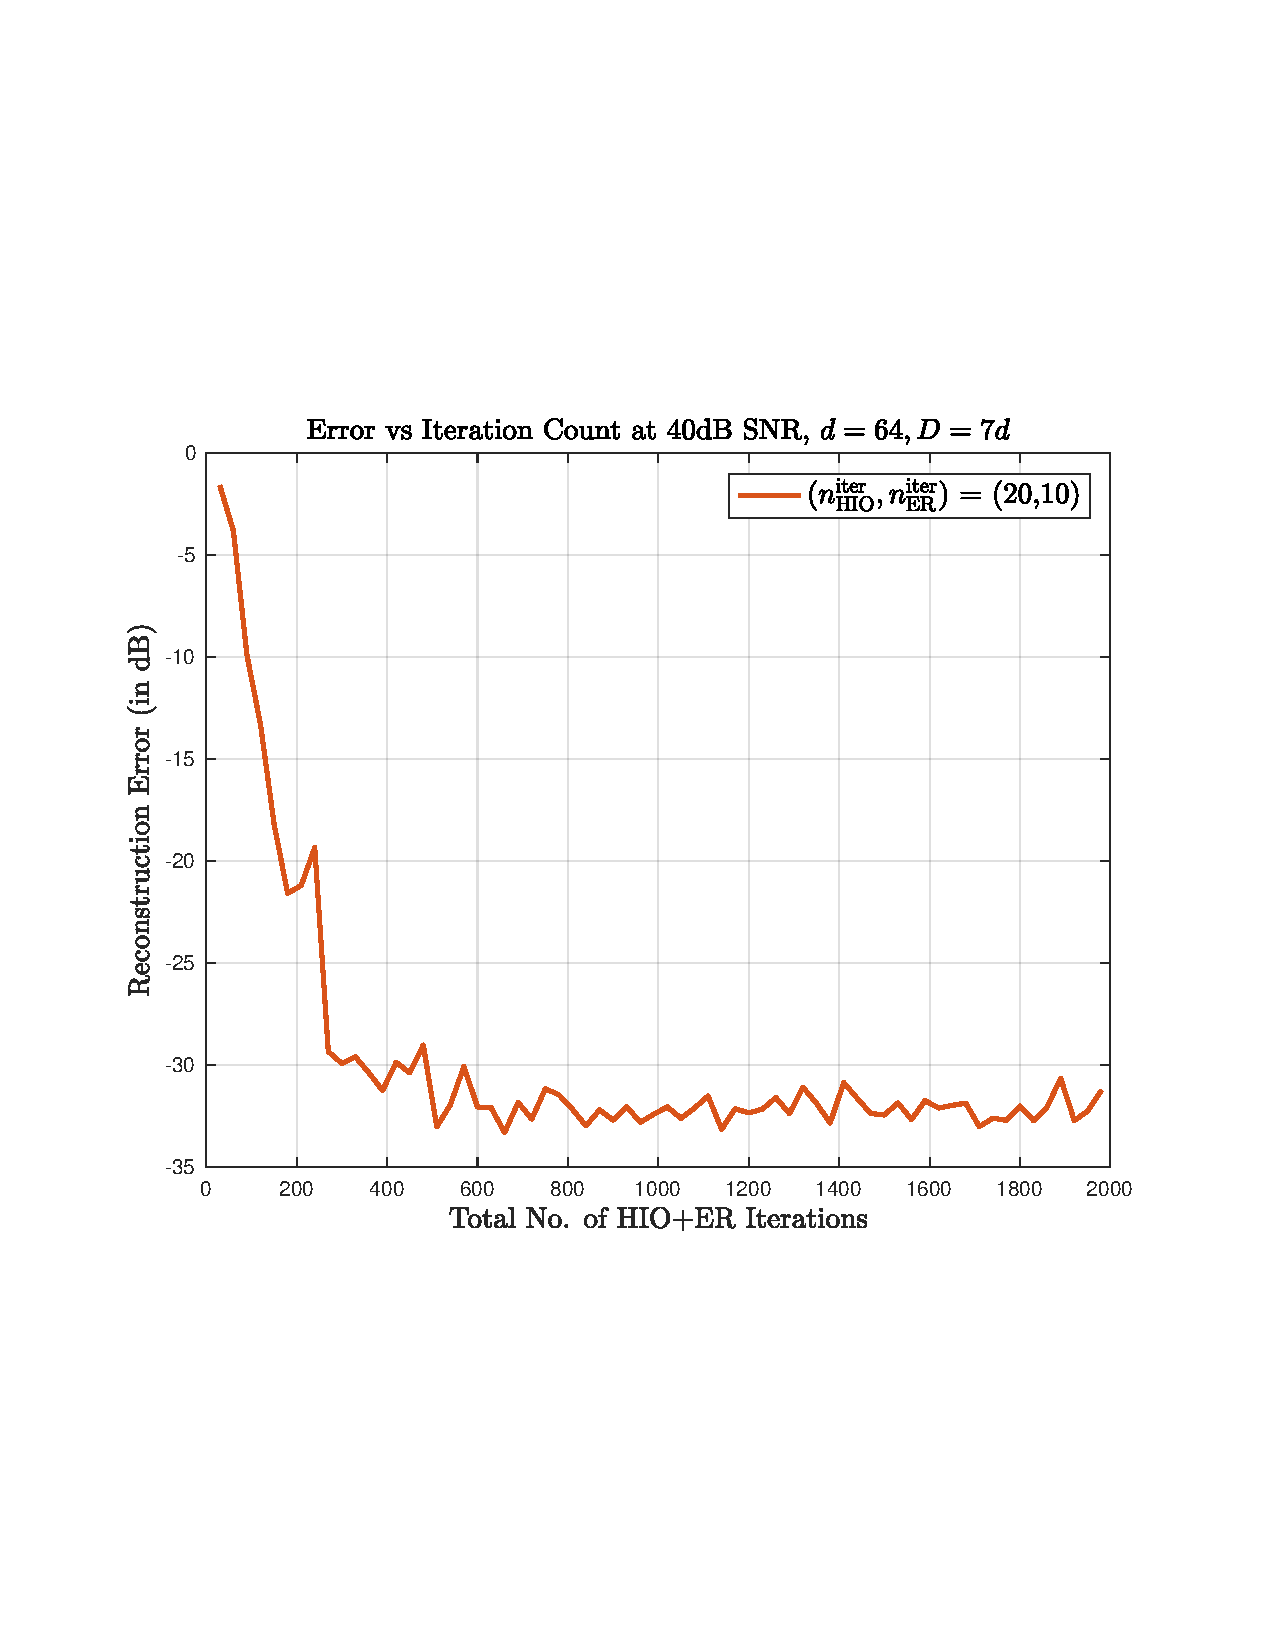
\includegraphics[clip=true, trim = 0.75in 2.75in 1in 2.75in,scale=0.45]{pics/err_iteration_count}
  \caption{Reconstruction Error vs. Iteration Count for HIO+ER Implementation}
  \label{fig:iter_HIOER}
\end{figure}
%-------------------------------------------------------

%SIMPLIFIED IN PARENTHESIS ABOVE?
%We refer the interested reader to \cite{bauschke2002phase} for an analysis
%of various alternating projection algorithms (including the aforementioned ER and HIO) from a convex
%optimization perspective -- our implementation of ER and HIO is inspired by this. 

We begin by presenting numerical results evaluating the robustness to measurement noise.  Figs.
\ref{fig:noise-7d} and \ref{fig:noise-15d} plot the error in reconstructing a $d=64$ length complex
vector $\x_0$ using $D=7d$ and $D=15d$ local correlation-based phaseless measurements respectively.
Note that this corresponds to using $\delta=4$ (and the associated $2\delta-1=7$ masks) and
$\delta=8$ (and the corresponding $2\delta-1=15$ masks) respectively. Moreover, the well-conditioned
{\em deterministic} (and sparse) measurement construction defined in Example 2 of Section
\ref{sec:MeasMatrix} was utilized along with additive Gaussian measurement noise. We see from Fig.
\ref{fig:noise-local} that the method proposed in this paper (denoted {\em BlockPR} in the figure)
performs reliably across a wide range of SNRs and compares favorably against existing popular phase
retrieval algorithms. When using a small number of measurements (as in Fig.  \ref{fig:noise-7d}, and
modeling real-world situations), both variants of the proposed method -- Alg.
\ref{alg:phaseRetrieval1}, as well as Alg.  \ref{alg:phaseRetrieval1} post-processed using $60$
HIO+ER iterations -- outperform the ER algorithm by significant margins and compare well with the 
popular HIO+ER algorithm. When more measurements are available (as in Fig.
\ref{fig:noise-15d}), the performance of the ER and HIO+ER algorithms approaches the performance of the
{\em BlockPR} variants proposed in this paper. In addition, the proposed methods also compare well
with the significantly more expensive {\em PhaseLift} reconstructions. We emphasize that the
superior performance of the proposed methods demonstrated here comes with rigorous theoretical
recovery guarantees for local measurements -- something that cannot
be said of any of the other methods in Fig.~\ref{fig:noise-local}. 

Additionally, Figs. \ref{fig:lowsnr_128} and \ref{fig:lowsnr_256} compare the performance of the
HIO+ER algorithm at low SNRs for problems sizes $d=128$ and $d=256$ respectively, with the various
{\em BlockPR} implementations -- including one with the improved magnitude estimation procedure
detailed in \S \ref{sec:MagEstImpNumerical} (with $s=1$ and using the average of the obtained
$\tilde D_{j\prime}$ block magnitude estimates). These figures demonstrate the value of the
magnitude estimation procedure from \S \ref{sec:MagEstImpNumerical} at low SNRs over the HIO+ER
post-processing method utilized in the other figures (and over the HIO+ER algorithm); we defer a
more detailed study of this to future work.

%
\begin{figure}[hbtp]
\centering
\begin{subfigure}[b]{0.8\textwidth}
\centering
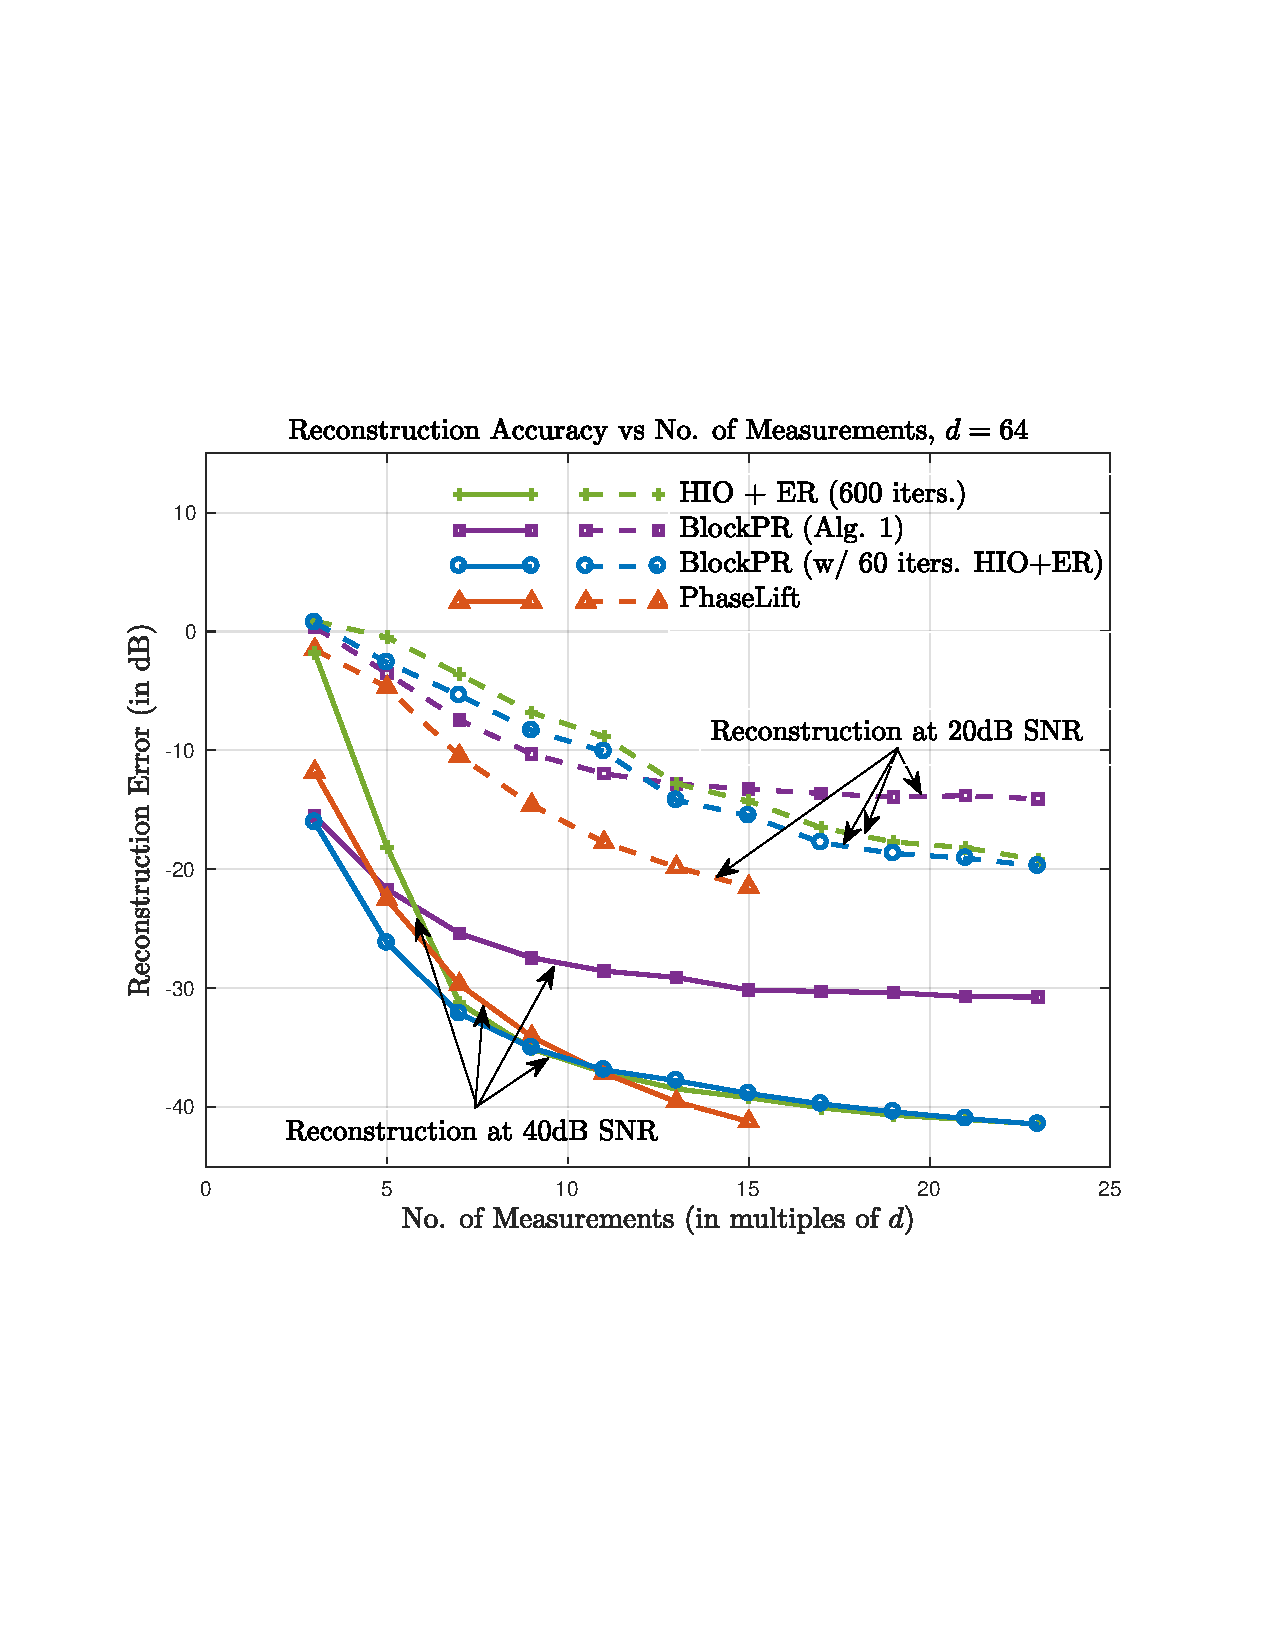
\includegraphics[clip=true, trim = 0.5in 2.5in 0.75in 2.5in,scale=0.55]{pics/fig5a}
%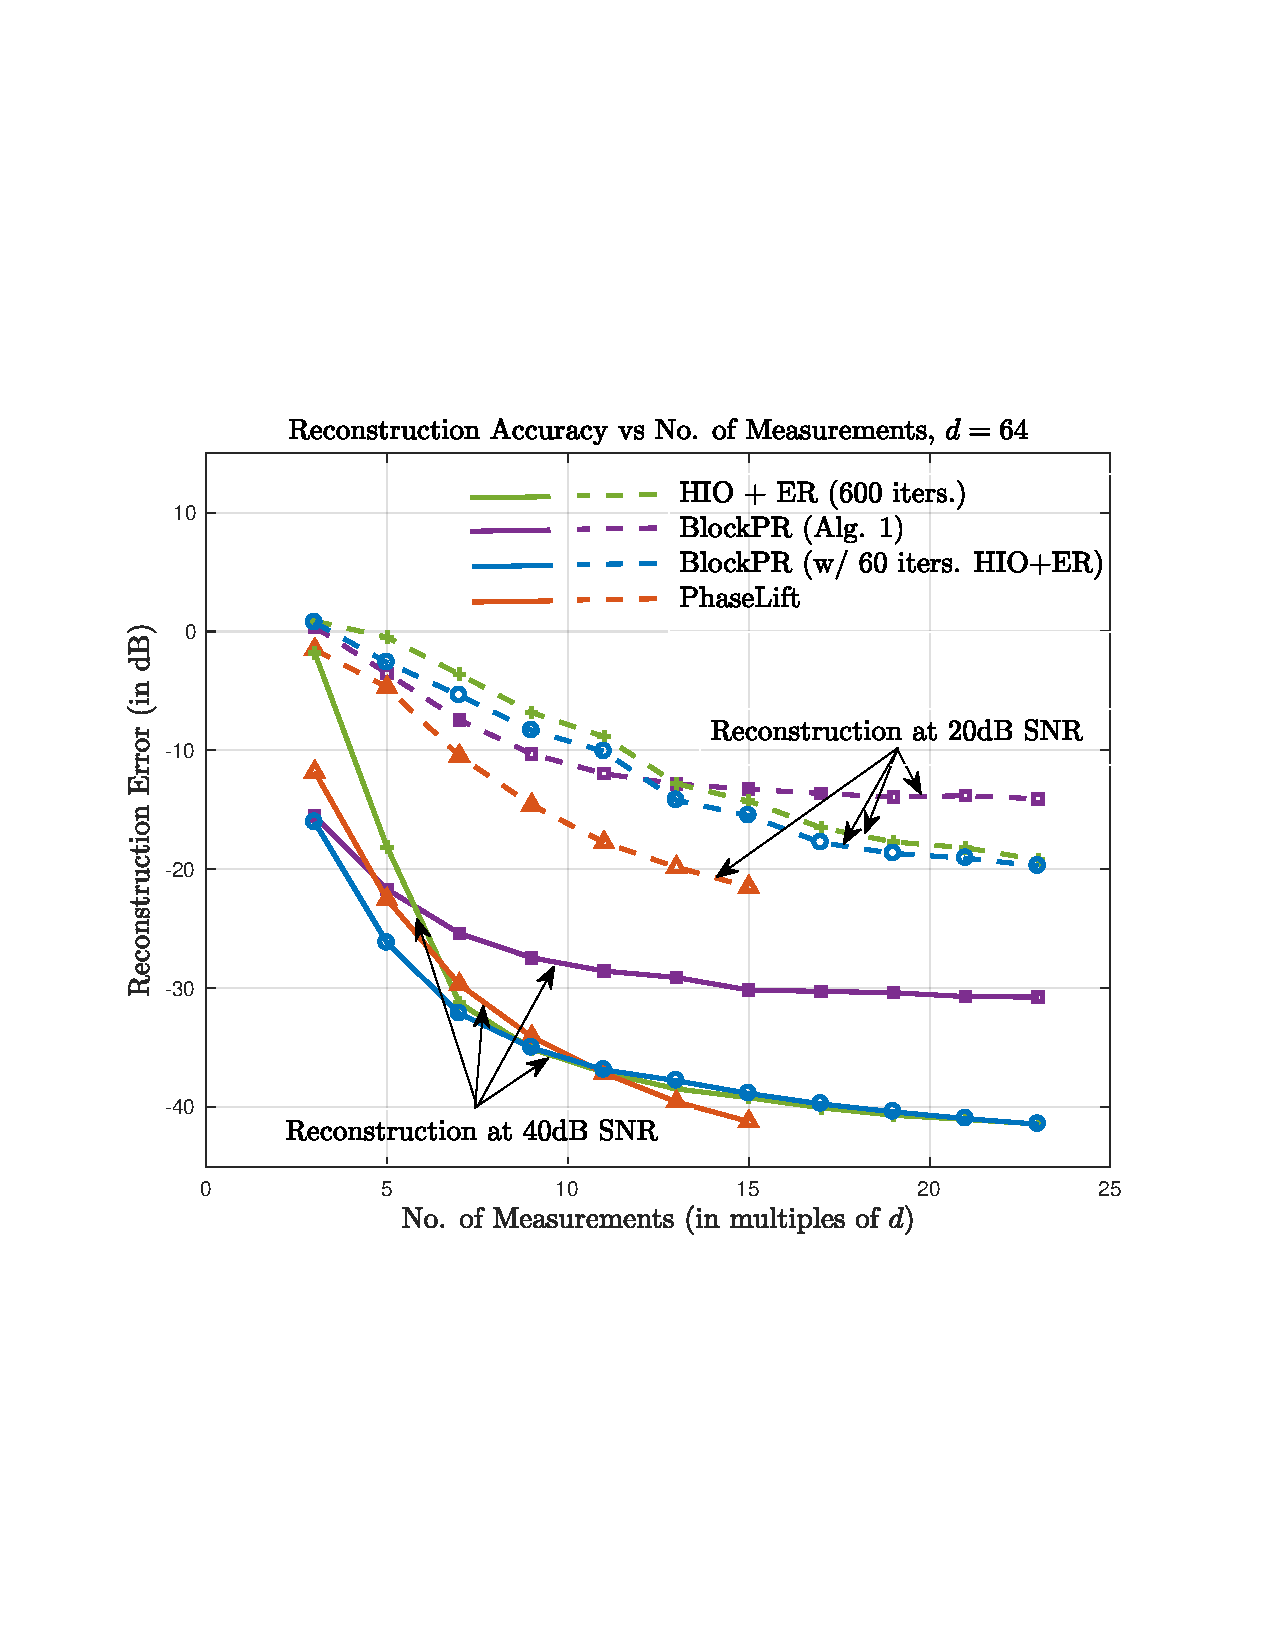
\includegraphics[clip=true, trim = 0.5in 2.5in 0.75in 2.5in,scale=0.42]{pics/measurements_600}
\caption{Reconstruction Error vs. No. of Measurements}
\label{fig:measurements}
\end{subfigure}

\begin{subfigure}[b]{0.8\textwidth}
\centering
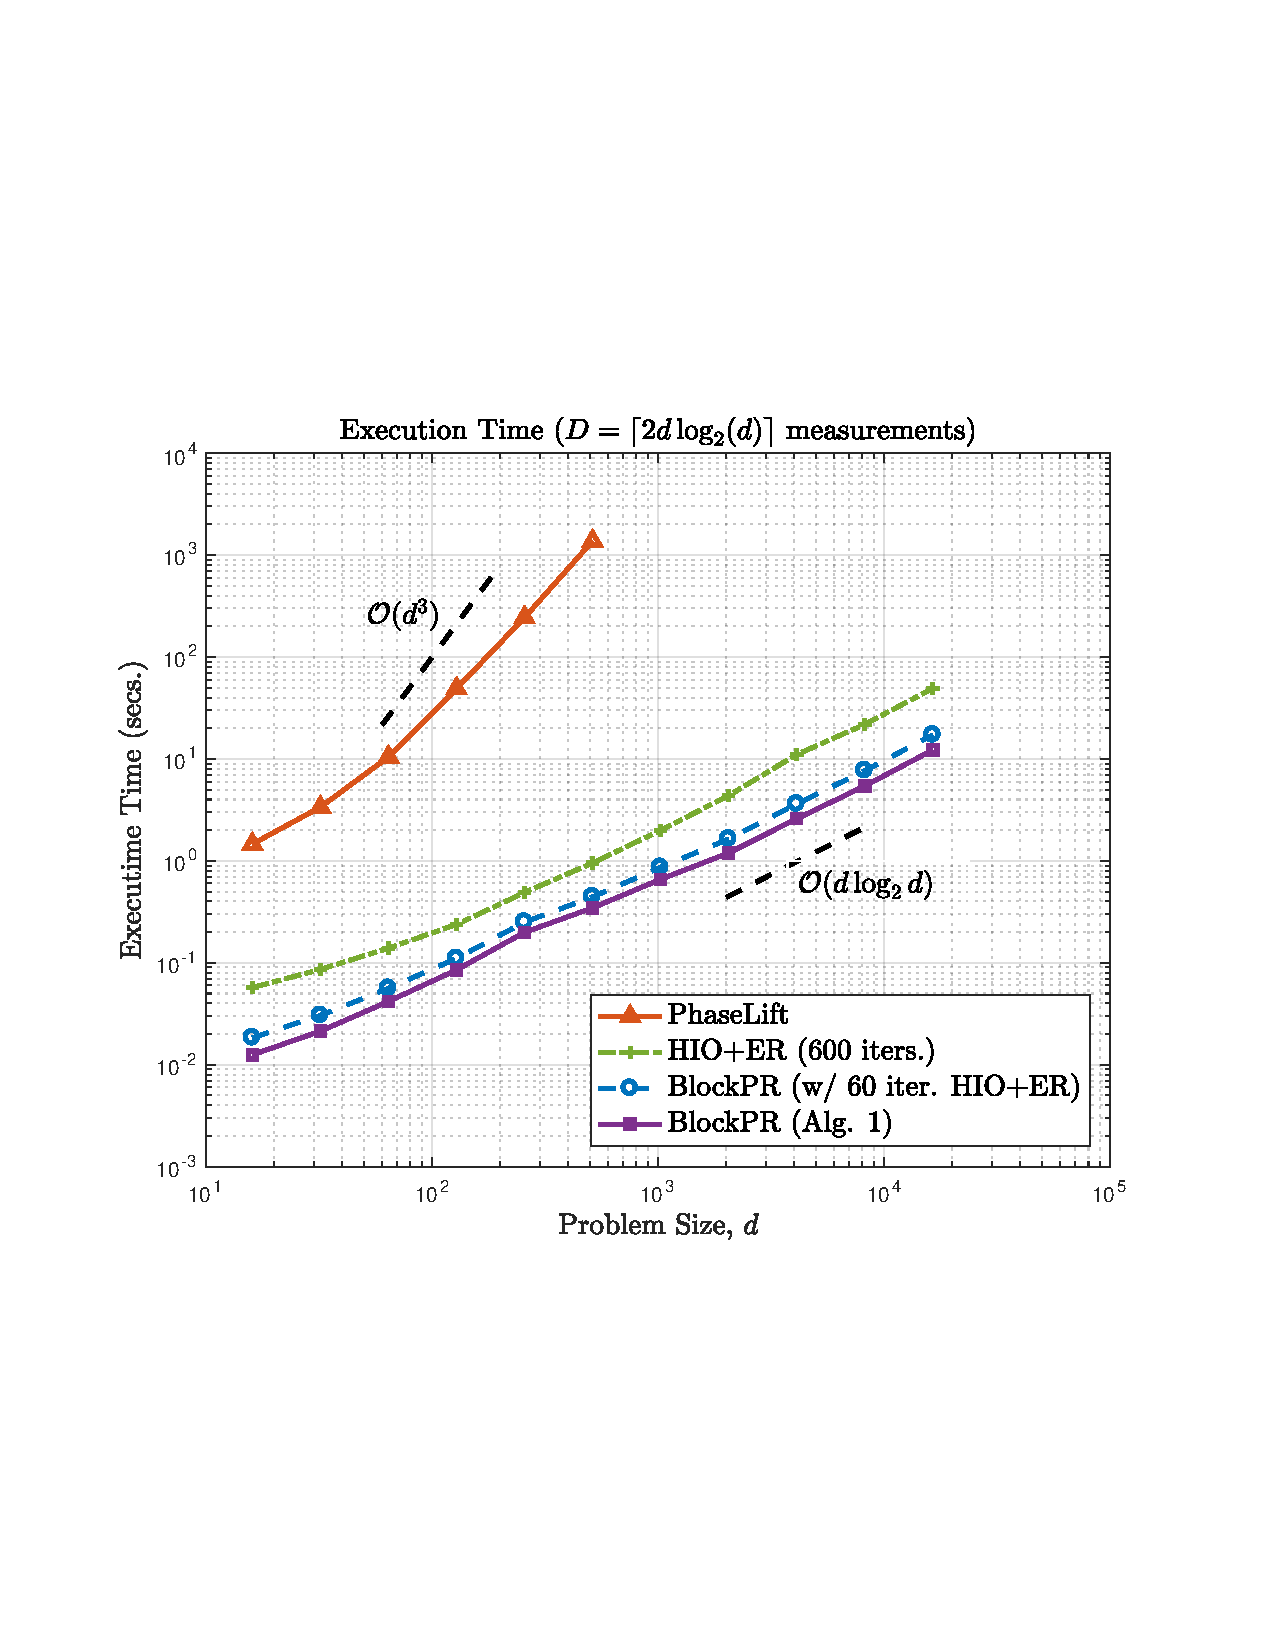
\includegraphics[clip=true, trim = 0.5in 2.5in 0.75in 2.5in,scale=0.55]{pics/fig5b}
\caption{Execution Time vs. Problem Size}
\label{fig:exectime}
\end{subfigure}
\caption{Performance Evaluation and Comparison of the Proposed Phase Retrieval Method 
(with Deterministic Local Correlation Measurements of Example 2, \S \ref{sec:MeasMatrix} and Additive Gaussian Noise)}
\label{fig:performance}
\end{figure}
%

Next, Fig. \ref{fig:measurements} plots the reconstruction error in recovering a $d=64$-length
complex vector as a function of the number of measurements used. This corresponds to using values of
$\delta$ ranging from $2$ to $12$ (and the associated $2\delta-1$ masks). As with Fig.
\ref{fig:noise-local}, the deterministic correlation-based measurement constructions of Section
\ref{sec:MeasMatrix} (Example construction $2$) were utilized along with an additive Gaussian noise
model. Plots are provided for simulations at two noise levels -- $20$ dB and $40$ dB. 
%For simplicity of visualization, we only plot results for the HIO alternating projection algorithm,
%{\em PhaseLift} and the two variants of the proposed algorithm (Alg. 1 and Alg. 1 w/ improved
%magnitude estimation and ER post-processing). 
Comparing the performance of the two {\em BlockPR} variants, we observe that the HIO+ER post-processing 
procedure provides improved reconstruction errors -- with the margin of improvement increasing when 
more measurements are available. We also notice that both variants of {\em BlockPR} compare
particularly well with the other algorithms (HIO+ER and {\em PhaseLift}) when small numbers of measurements are available.
%Additionally, when the improved magnitude estimation procedure is utilized, the proposed method is almost as
%accurate as the significantly more expensive {\em PhaseLift} algorithm and outperforms the popular 
%HIO algorithm by sometimes significant margins. 
%At the $40$ dB (moderate) noise 
%level, the proposed method provides the best reconstruction accuracy when approximately $7d$ or
%fewer measurements are available. 

Finally, Fig. \ref{fig:exectime} plots the average execution time (in seconds) required to solve the
phase retrieval problem using $D = \lceil 2d\log_2d\rceil$ measurements. For comparison, execution
times for the {\em PhaseLift} and HIO+ER alternating projection algorithms are provided. We observe
that both variants of the proposed method are several orders of magnitude faster than the {\em
PhaseLift} algorithm,\footnote{\ For computational efficiency and due to memory constraints, the {\em
PhaseLift} plot in Fig. \ref{fig:exectime} was generated using the TFOCS software package
(http://cvxr.com/tfocs/) instead of the more computationally expensive CVX software package.} and between
$2$--$5$ times faster than the HIO+ER implementation. Moreover, the plot illustrates the essentially
FFT-time computational complexity (see \S \ref{sec:RuntimeAlg1}) of the proposed method. Between the
two {\em BlockPR} variants, we see that there is a small trade-off between reduced execution time and
improved accuracy; one of the two variants may be more appropriate depending on the application
requirements.

\subsection{Experiments with Ptychographic Measurements from Example 1 of \S \ref{sec:MeasMatrix}}
\label{sec:PtychographicMeasExper}

%
\begin{figure}[hbtp]
\centering
\begin{subfigure}[b]{0.8\textwidth}
\centering
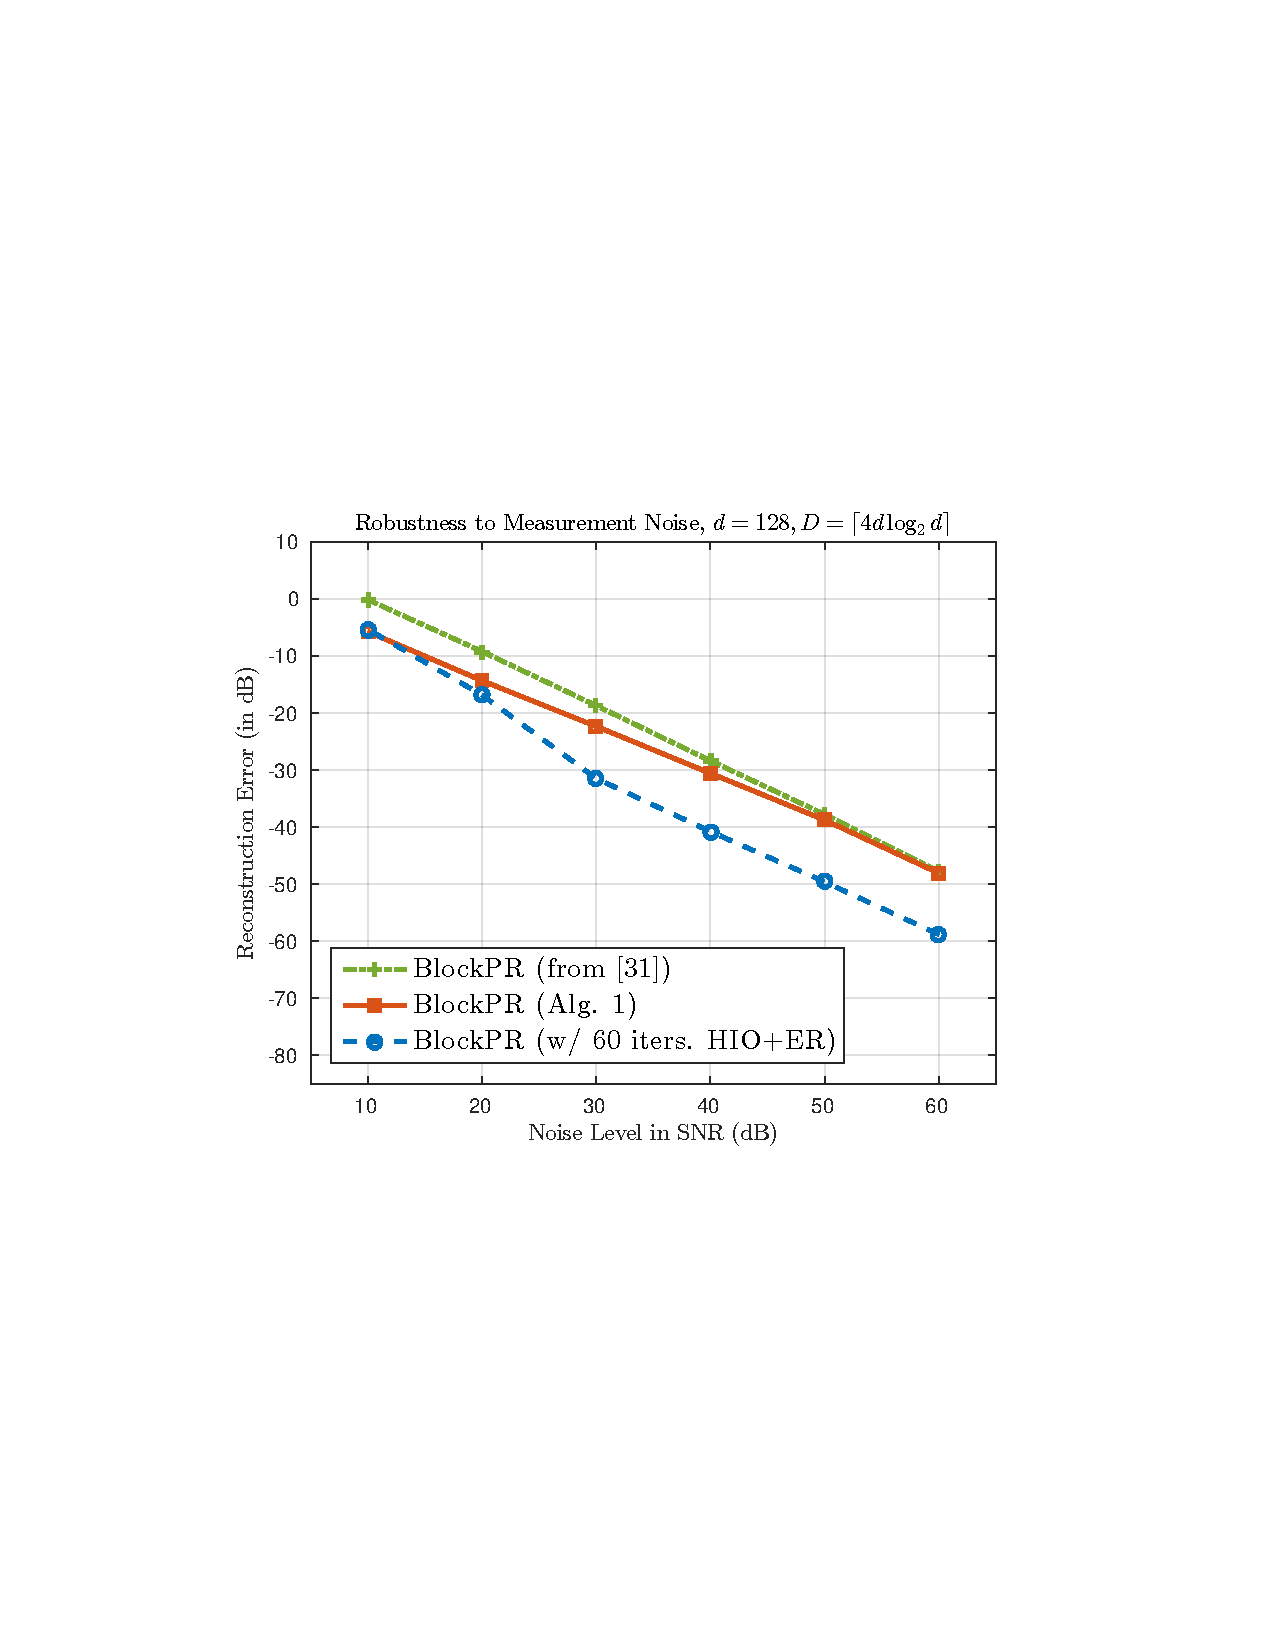
\includegraphics[clip=true, trim = 1.5in 3.35in 1.6in 3.25in,scale=0.8]{pics/fig6a}
\caption{Improved Robustness to Measurement Noise -- Comparing Variants of the {\em BlockPR}
algorithm}
\label{fig:global_vs_local_ptych}
\end{subfigure}
\hfill
\begin{subfigure}[b]{0.8\textwidth}
\centering
%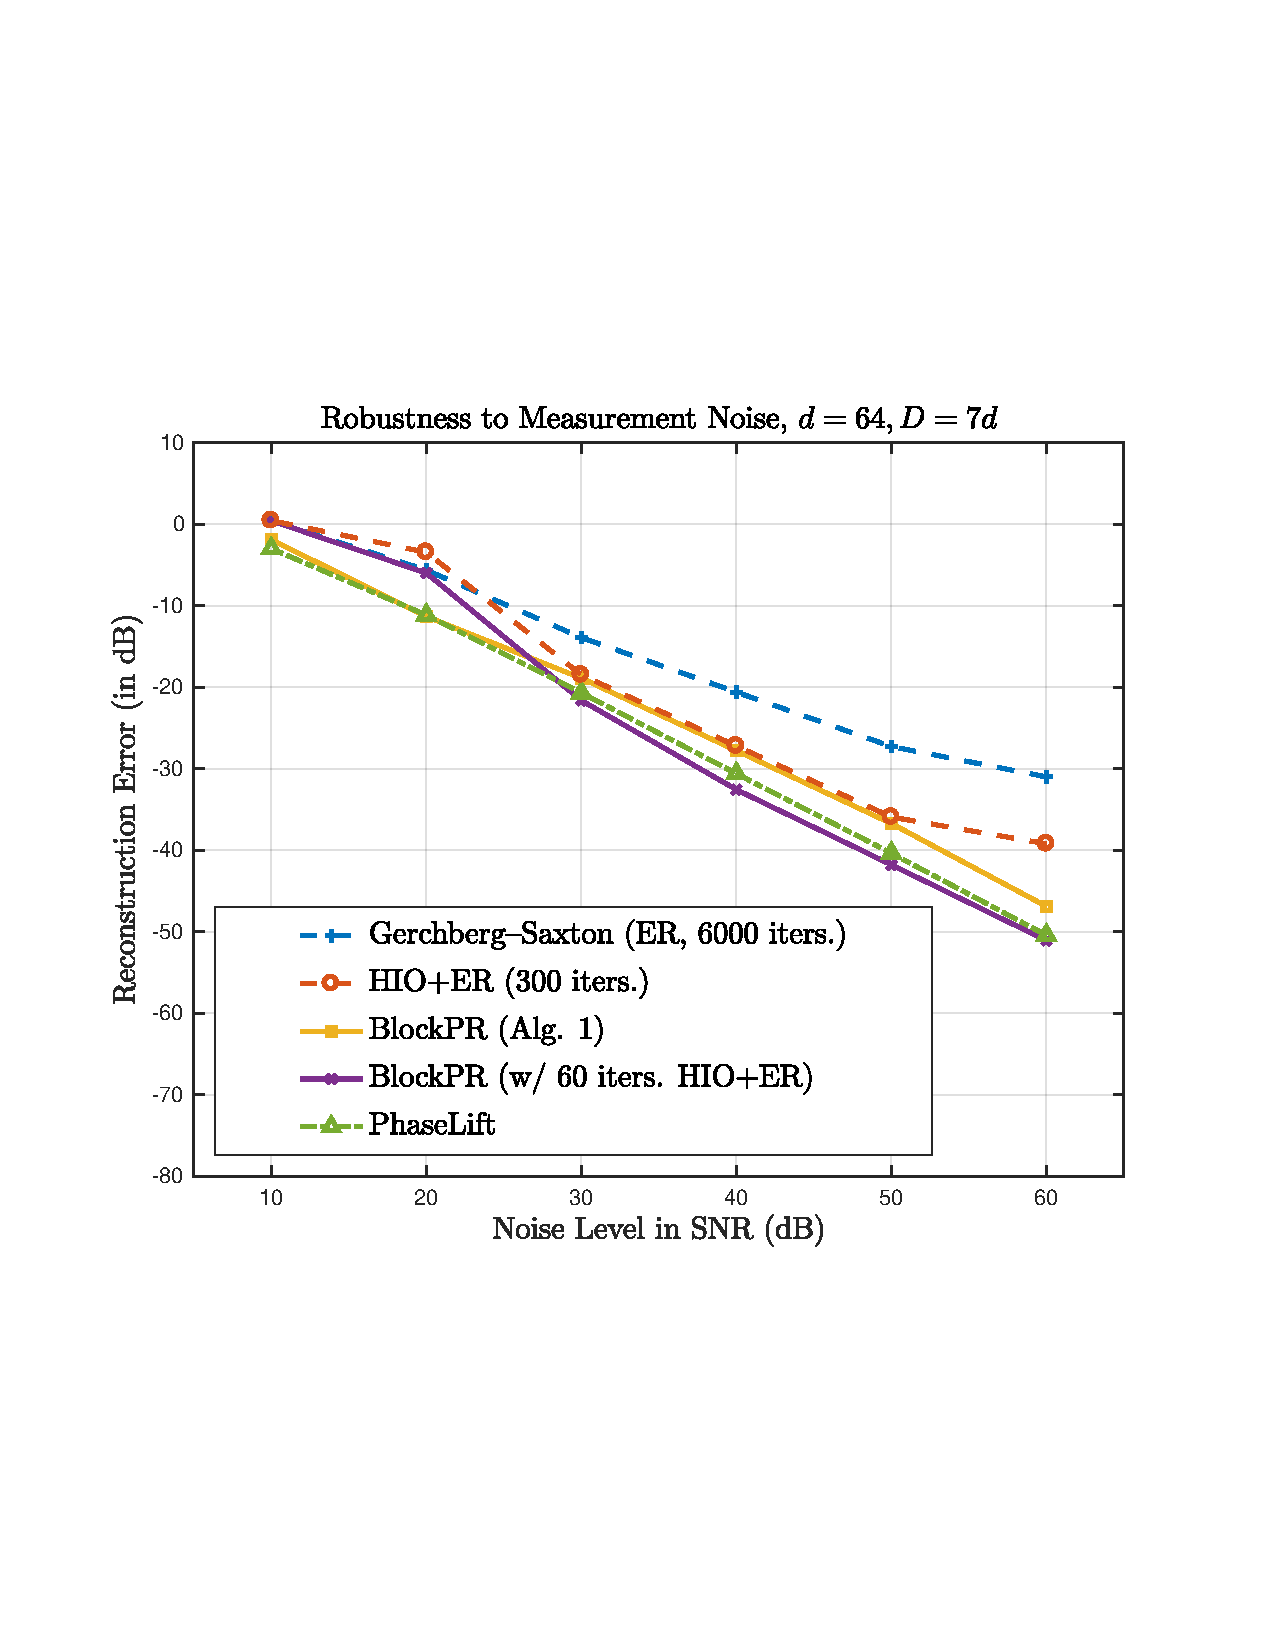
\includegraphics[clip=true, trim = 0.75in 2.75in 1in 2.5in,scale=0.45]{pics/fig6b}
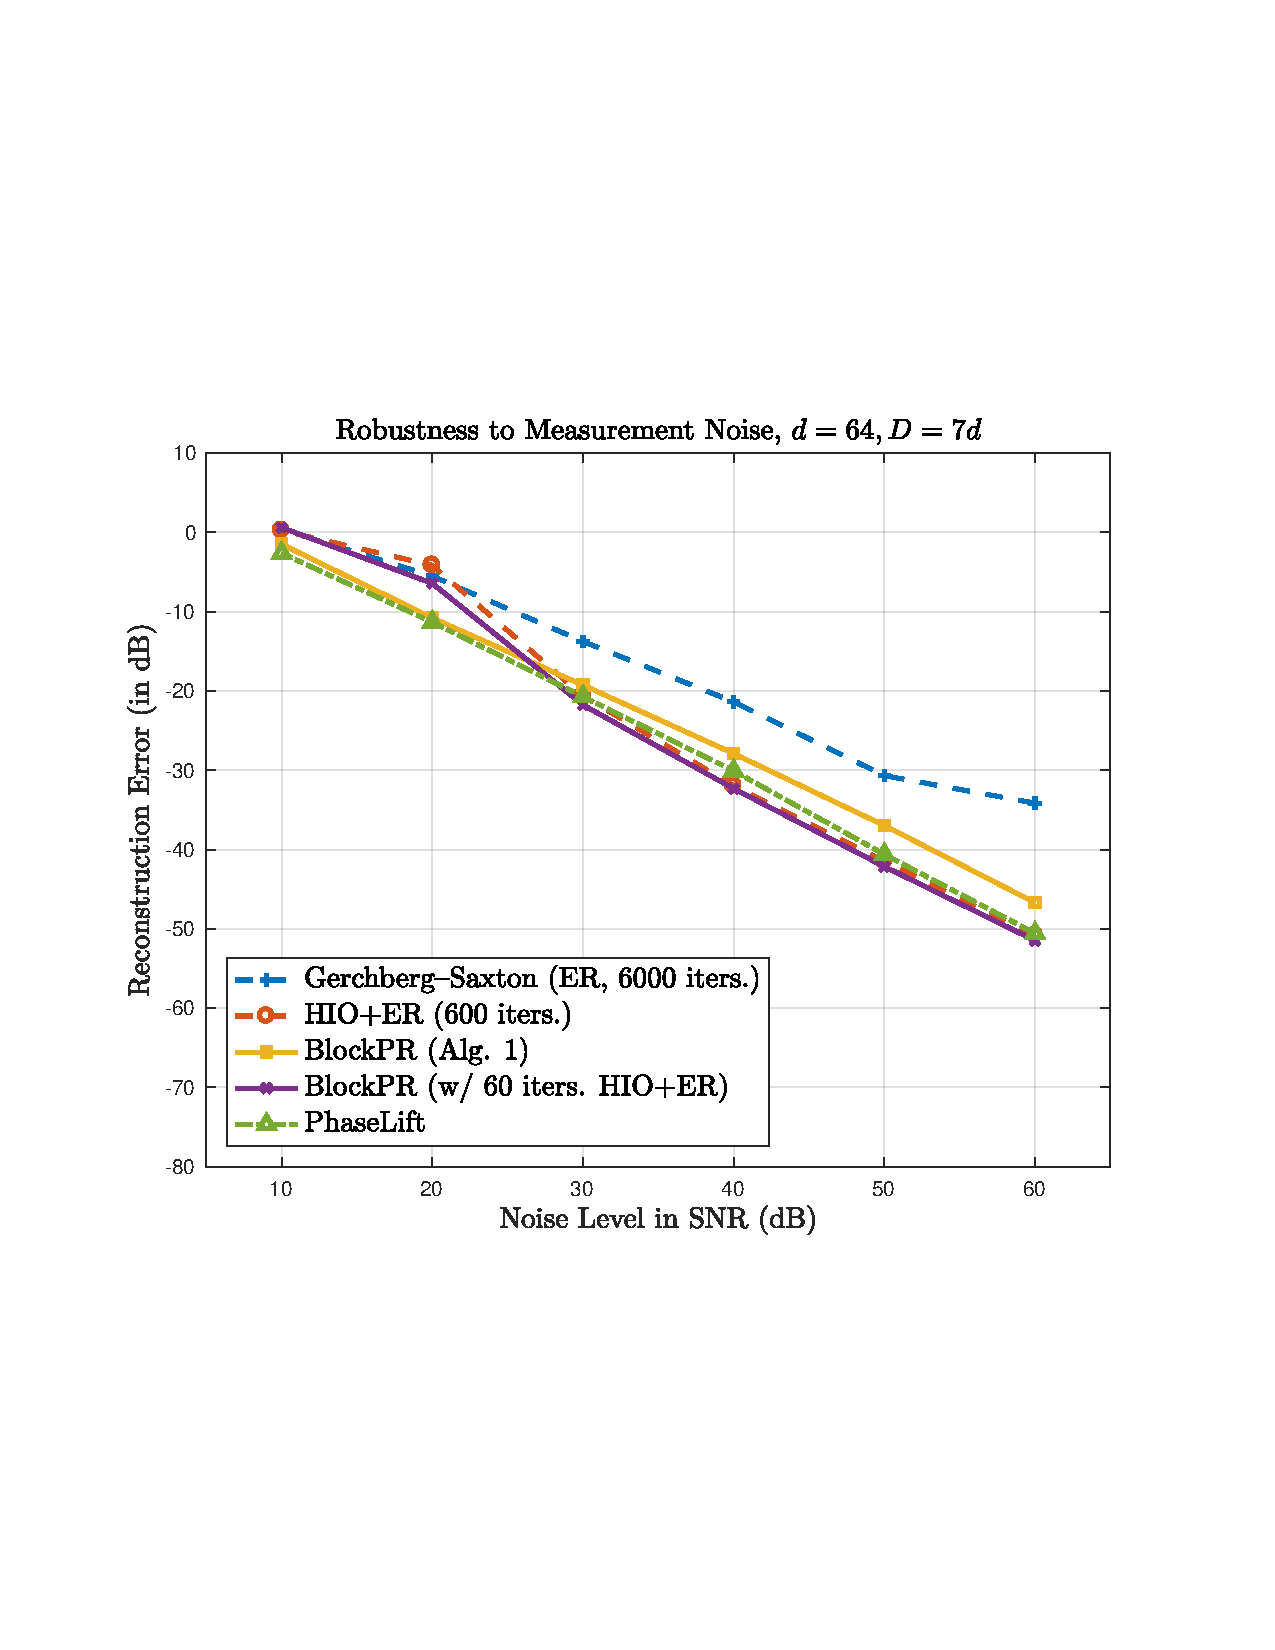
\includegraphics[clip=true, trim = 0.75in 2.75in 1in 2.5in,scale=0.6]{pics/robustness600_Fourier}
\caption{Phase Retrieval from $D=7d$ Measurements -- Comparison with Other Phase Retrieval Algorithms}
\label{fig:noise_robust_ptych}
\end{subfigure}
\caption{Numerical Evaluation of the Proposed Algorithm with the Ptychographic Measurements from
    Example 1 of \S \ref{sec:MeasMatrix}}
\label{fig:ptych_meas}
\end{figure}
%
%We now present a selection of empirical results demonstrating the accuracy, robustness and
%efficiency of the proposed method when using the ptychographic measurements from Example 1, \S
%\ref{sec:MeasMatrix}, while also noting that the qualitative and quantitative nature of the other
%results are similar to those presented in \S \ref{sec:SparseMeasureMasks}.  
{ We now present a selection of empirical results demonstrating the accuracy, robustness, and efficiency of the proposed method when using the ptychographic measurements from Example 1, \S\ref{sec:MeasMatrix} and observe that, in this case, the comparison between the proposed algorithm and existing methods is similar to that in section \S\ref{sec:SparseMeasureMasks}.}  Recall that (see Example 1 from \S \ref{sec:MeasMatrix} and \S \ref{sec:conn_pty} for details) this measurement construction
corresponds to a discretization of the ptychographic measurements $\left|\mathcal{F}[\widetilde h
\cdot S_l f](\omega) \right|^2$ as per \eqref{eq:ptych}, where $f$ is the unknown specimen and
$\widetilde h(t) = \frac{e^{-t/a}}{\sqrt[4]{2\delta -1}}$ denotes the {\em single, deterministic}
illumination function (or mask). As before, $\delta$ defines the local support of the illumination
function and we consider a discretization involving $2\delta-1$ Fourier modes and sample/specimen
shifts of $1$ unit or pixel (yielding a total of $d$ shifts in the discrete problem formulation). 

We begin with Fig. \ref{fig:global_vs_local_ptych}, which demonstrates the relative performance of
the {\em BlockPR} variants described in \cite{IVW2015_FastPhase} and this paper. More specifically,
we plot the error in reconstructing a $d=128$ length complex Gaussian test signal using $D = \lceil
4d\log_2 d\rceil$ measurements at different added noise levels. As with Fig.
\ref{fig:eig_vs_greedy}, we plot results for three different variants of the {\em BlockPR}
algorithm: (i) Algorithm \ref{alg:phaseRetrieval1}, (ii) Algorithm \ref{alg:phaseRetrieval1} with
the HIO+ER post-processing procedure as described in \S \ref{sec:SparseMeasureMasks}, and (iii) the implementation
from \cite{IVW2015_FastPhase}. We again observe (as in Fig. \ref{fig:eig_vs_greedy}) that the methods
described in this paper (which use eigenvector-based angular synchronization) are more accurate than
that detailed in \cite{IVW2015_FastPhase} (which uses a greedy angular synchronization method), with
the improvement in performance being especially significant at low SNRs. Next, Fig.
\ref{fig:noise_robust_ptych} studies the performance of the proposed method(s) against three other
popular phase retrieval algorithms -- {\em PhaseLift}, the {\em Gerchberg--Saxton} Error Reduction
(ER) algorithm, and the Hybrid Input--Output (HIO) algorithm (with implementation parameters identical to those in 
\S \ref{sec:SparseMeasureMasks}). As with Fig. \ref{fig:noise-7d}, we
consider the reconstruction of a $d = 64$ length complex vector $x_0$ using $D = 7d$ measurements in
the presence of additive Gaussian noise. We observe that the methods proposed in this paper outperform the 
ER algorithm and compare very well with the HIO+ER and (the significantly more expensive) {\em PhaseLift} 
algorithms across a wide range of SNRs. 
%While there may be an optimal set of
%algorithmic parameters which improve the convergence of the ER and HIO algorithms, the selection of
%such parameters is not immediately obvious. 
Finally, we note that the execution time plot for this
ptychographic measurement construction is qualitatively and quantitatively similar to Fig.
\ref{fig:exectime} -- the proposed methods are faster (by a factor of $2$--$5$) than an equivalent HIO+ER
implementation and orders of magnitude faster than convex optimization approaches such as {\em
PhaseLift}. 

%Moreover, the interested reader is
%encouraged to download the open source code implementing these results at \cite{bitbucket_BlockPR}
%and run their own experiments. \textcolor{red}{add exec time plot or just say it is the same as in
%Fig. 4b?} Finally, we plot the execution time
%-- NOTE:  HIO and ER as convex opt. ref. -- -- A reformulation of ER and HIO as convex optimization methods, probably worth a closer read -- also justifies Aditya's HIO implementation \cite{bauschke2002phase}\\
